\documentclass[12pt,a4paper]{report}

% ---------- Packages ----------
\usepackage[margin=2.5cm]{geometry}
\usepackage{iftex}
\ifPDFTeX
  \usepackage[T1]{fontenc}
  \usepackage[utf8]{inputenc}
  \usepackage{lmodern}
\else
  \usepackage{fontspec}
  \setmainfont{Arial} % or Calibri if installed
\fi
\usepackage{setspace}
\onehalfspacing
\raggedbottom

\usepackage{graphicx}
\usepackage{float}
\usepackage{caption}
\usepackage{array}
\usepackage{booktabs}
\usepackage{longtable}
\usepackage{tabularx}
\usepackage{amsmath}
\usepackage{amssymb}
\usepackage[hidelinks,hypertexnames=false]{hyperref}
\usepackage{fancyhdr}
\usepackage{titlesec}
\usepackage{tocloft}

% ---------- Header / Footer ----------
\pagestyle{fancy}
\fancyhf{}
\fancyhead[L]{\leftmark}
\fancyfoot[L]{PFA -- 4th year GL / IA}
\fancyfoot[R]{\thepage}
\setlength{\headheight}{15pt}

% ---------- Chapter formatting ----------
\titleformat{\chapter}[display]
{\bfseries\Large}
{\chaptername\ \thechapter}
{0.75em}
{\Huge}
\titlespacing*{\chapter}{0pt}{0pt}{1.5ex}
\titlespacing*{\section}{0pt}{1.5ex plus 0.5ex minus 0.2ex}{0.8ex}
\titlespacing*{\subsection}{0pt}{1.2ex plus 0.4ex minus 0.2ex}{0.6ex}

% ---------- Line breaking ----------
\hyphenpenalty=10000
\exhyphenpenalty=10000
\tolerance=2000
\emergencystretch=3em
\righthyphenmin=62
\lefthyphenmin=62
\hbadness=10000
\vbadness=10000
\hfuzz=5pt
\vfuzz=5pt

% ---------- Document ----------
\begin{document}

% ---------- Cover Page ----------
\begin{titlepage}
    \centering
    \vspace*{1cm}

    {\Large EPI Educational Group}\\[0.5cm]
    {\large Department / Track: GL -- IA/DS}\\[2cm]

    {\Huge \textbf{Project Title}}\\[1cm]
    {\Large PFA Report}\\[2cm]

    \begin{flushleft}
    \textbf{Student(s):} Name 1, Name 2\\
    \textbf{Supervisor:} Supervisor Name\\
    \textbf{Academic Year:} 2024/2025\\
    \textbf{Date:} Month Year
    \end{flushleft}

    \vfill
\end{titlepage}

% ---------- Preliminary Pages ----------
\pagenumbering{roman}
\chapter*{Acknowledgements}
\phantomsection
\addcontentsline{toc}{chapter}{Acknowledgements}

We would like to express our sincere gratitude to everyone who contributed to the completion of this project.

First, we would like to thank our supervisor for their valuable guidance, support, and advice throughout the development of this work.

We also extend our thanks to the faculty members and staff of EPI for providing us with the knowledge, resources, and environment necessary for the realization of this project.

Special thanks go to our friends and colleagues for their encouragement, collaboration, and constructive feedback during the different stages of the project.

Finally, we would like to express our deepest gratitude to our families for their continuous support, patience, and motivation throughout our academic journey.
\chapter*{Abstract}
\phantomsection
\addcontentsline{toc}{chapter}{Abstract}
This project presents the design and development of \textbf{BViral Control Center}, an intelligent web platform for social media content management and AI‑powered video processing. The system allows creators and administrators to manage accounts, schedule and publish posts across multiple platforms, monitor analytics, and receive operational alerts through a unified dashboard.

The platform also integrates an AI Video Studio that performs video enhancement, automatic subtitle generation, and content performance prediction. A multimodal AI pipeline was built using visual, audio, and textual features extracted from short‑form videos. These features are used to train predictive models that estimate a video’s expected reach and engagement prior to publication.

The system architecture was formalized using UML use‑case, class, and sequence diagrams to capture both functional requirements and structural design. Overall, the solution combines modern web technologies, cloud‑based services, and advanced AI tools to deliver a scalable environment for digital content optimization.

\textbf{Keywords:} Social Media Management, Artificial Intelligence, Video Enhancement, Machine Learning, Content Scheduling
\chapter*{Résumé}
\phantomsection 
Ce projet présente la conception et le développement de \textbf{BViral Control Center}, une plateforme web intelligente dédiée à la gestion de contenu sur les réseaux sociaux et au traitement vidéo assisté par l’intelligence artificielle. Elle permet aux créateurs et administrateurs de gérer plusieurs comptes, planifier et publier des contenus, suivre les statistiques, et recevoir des alertes via un tableau de bord centralisé.

La plateforme intègre également un \emph{AI Video Studio} capable d’améliorer la qualité des vidéos, de générer automatiquement des sous‑titres et de prédire la performance d’un contenu avant publication. Un pipeline multimodal a été mis en place pour extraire des caractéristiques visuelles, audio et textuelles à partir de vidéos courtes. Ces caractéristiques alimentent des modèles d’apprentissage automatique destinés à estimer la portée et l’engagement futurs.

L’architecture du système a été formalisée à l’aide de diagrammes UML (cas d’usage, classes, séquences) afin de définir les aspects fonctionnels et structurels de l’application. La solution combine des technologies web modernes, des services cloud et des outils d’IA avancés pour offrir un environnement évolutif et performant dédié à l’optimisation du contenu numérique.


\clearpage
\tableofcontents
\clearpage
\listoffigures
\clearpage
\listoftables
\clearpage  
\chapter*{Glossary / List of Abbreviations}
\phantomsection
\addcontentsline{toc}{chapter}{Glossary / List of Abbreviations}

\begin{longtable}{|p{4cm}|p{10cm}|}
\hline
\textbf{Acronym} & \textbf{Meaning} \\
\hline
API & Application Programming Interface \\
UML & Unified Modeling Language \\
AI & Artificial Intelligence \\
ML & Machine Learning \\
XAI & Explainable Artificial Intelligence \\
EDA & Exploratory Data Analysis \\
PCA & Principal Component Analysis \\
XGBoost & eXtreme Gradient Boosting \\
RF & Random Forest \\
LGBM & Light Gradient Boosting Machine \\
SHAP & SHapley Additive exPlanations \\
LLM & Large Language Model \\
NLP & Natural Language Processing \\
ASR & Automatic Speech Recognition \\
GAN & Generative Adversarial Network \\
GPU & Graphics Processing Unit \\
CPU & Central Processing Unit \\
RAM & Random Access Memory \\
OOM & Out Of Memory \\
ORM & Object Relational Mapping \\
JWT & JSON Web Token \\
RLS & Row-Level Security \\
OAuth & Open Authorization \\
PKCE & Proof Key for Code Exchange \\
CRUD & Create, Read, Update, Delete \\
REST & Representational State Transfer \\
KPI & Key Performance Indicator \\
RMSE & Root Mean Square Error \\
MAE & Mean Absolute Error \\
MFCC & Mel-Frequency Cepstral Coefficients \\
RMS & Root Mean Square \\
FPS & Frames Per Second \\
PSNR & Peak Signal-to-Noise Ratio \\
SSIM & Structural Similarity Index Measure \\
LPIPS & Learned Perceptual Image Patch Similarity \\
WAV & Waveform Audio File Format \\
SRT & SubRip Subtitle Format \\
JSON & JavaScript Object Notation \\
CSV & Comma-Separated Values \\
HTTP & HyperText Transfer Protocol \\
SQL & Structured Query Language \\
IDE & Integrated Development Environment \\
FFmpeg & Fast Forward Moving Picture Experts Group \\
CRISP-DM & Cross-Industry Standard Process for Data Mining \\
\hline
\end{longtable}

% ---------- Main Report ----------
\clearpage
\pagenumbering{arabic}
\chapter*{General Introduction}
\phantomsection
\addcontentsline{toc}{chapter}{General Introduction}

\noindent In the contemporary digital era, social media has transformed from a mere communication tool into a vital business infrastructure for content creators, influencers, digital marketers, and global enterprises[cite: 28]. Establishing and maintaining a successful online presence currently demands active participation across a diverse ecosystem of platforms, including YouTube, TikTok, Instagram, Facebook, and Snapchat[cite: 29]. However, this multi-platform reality introduces immense logistical and technical challenges[cite: 29]. Content creators are forced to fracture their workflows, shifting continuously between separate interfaces to manage accounts, schedule publications, edit multi-format assets, and decipher disjointed performance analytics[cite: 29]. 

Compounding these operational hurdles is the relentless evolution of recommendation algorithms[cite: 104]. Creators frequently lack data-driven, pre-publishing insights, leaving them to rely on trial-and-error rather than predictive intelligence to estimate content reach and audience engagement[cite: 95, 96]. Furthermore, short-form video content demands high production value to capture immediate viewer attention, yet professional video enhancement tools remain largely confined to expensive, standalone desktop applications isolated from publishing platforms[cite: 35, 37]. This operational fragmentation and systemic lack of algorithmic foresight constitute the primary problem statement driving this project[cite: 105].

To bridge these prominent technological gaps, this project introduces the design and development of the \textbf{BViral Control Center}[cite: 6]. The principal objective of this work is to build an intelligent, centralized web platform that unifies comprehensive social media management with state-of-the-art, AI-powered video processing and predictive analytics[cite: 6, 7]. By engineering a single, cohesive dashboard, the solution aims to:
\begin{itemize}
    \item Centralize multi-platform account synchronization using secure, modern OAuth 2.0 and PKCE communication protocols[cite: 57, 58, 71].
    \item Automate content publication through an integrated scheduling system backed by visual calendars and asynchronous background job queues[cite: 61, 73].
    \item Provide comprehensive cross-platform analytics to track aggregated key performance indicators (KPIs) and revenue metrics[cite: 64, 65].
    \item Embed an AI Video Studio capable of video quality upscaling, facial restoration, automated speech-to-text subtitling, and timeline video editing[cite: 8, 66, 68].
    \item Deploy a Pre-Posting Predictive Agent trained on multimodal content features to act as an algorithmic coach, providing actionable view-count forecasting and structural feedback before publishing[cite: 8, 9, 96].
\end{itemize}

\noindent To guarantee both software reliability and data science rigor, a dual-methodology approach was adopted[cite: 78]. The architectural and full-stack software development lifecycle is governed by the engineering discipline of the \textbf{V-Model}[cite: 78, 79]. This framework mandates clear traceability by linking every conceptual phase (from requirement specifications to system architecture) with a corresponding verification and testing stage, effectively minimizing integration risks across the platform's multiple tiers[cite: 82, 84, 89]. Concurrently, the machine learning components follow the iterative \textbf{CRISP-DM} (Cross-Industry Standard Process for Data Mining) lifecycle[cite: 78, 93]. This structured data pathway handles the project from initial business understanding through multimodal data ingestion, feature compression using Principal Component Analysis (PCA), regression model training using eXtreme Gradient Boosting (XGBoost), and final backend integration[cite: 95, 99, 100, 103].

\noindent This report outlines the complete realization of the platform and is structured into four distinct chapters[cite: 16, 18]:
\begin{itemize}
    \item \textbf{Chapter 1: State of the Art} presents the general context and details the problem statement[cite: 27, 28]. It includes a comparative study and critique of existing commercial solutions, outlines the core theoretical AI and software concepts, defines system actors, and provides an in-depth justification of the project's dual working methodologies[cite: 27, 42, 57, 78].
    \item \textbf{Chapter 2: Requirements Analysis and Data Specification} models the structural and behavioral dynamics of the platform[cite: 111]. This section maps functional and non-functional requirements through comprehensive UML use-case descriptions, a type-safe class data model, and detailed sequence diagrams for critical flows like authentication and automated post publishing, alongside the technical specification of the AI pipeline[cite: 11, 157, 159, 160].
    \item \textbf{Chapter 3: System Design and Realisation} exposes the technical architecture and choices underlying the software[cite: 163]. It illustrates the layout of the pnpm monorepo, details the client-server layer (React/Vite frontend, Fastify REST API, and PostgreSQL/Supabase database), details the Python-based computer vision stack, and demonstrates the final realized user interfaces[cite: 165, 170, 171].
    \item \textbf{Chapter 4: AI Component: Experiments and Evaluation} details the data science operations and empirical results[cite: 16, 18]. It covers the ingestion of short-form video datasets, exploratory data analysis, acoustic and semantic feature extraction via Whisper and Llama 3, regression modeling performance comparisons, and model explainability using SHapley Additive exPlanations (SHAP)[cite: 56, 91, 97, 100, 155].
\end{itemize}
Finally, a global conclusion synthesizes the achieved results and proposes valuable future perspectives for expansion[cite: 18].
\chapter{State of the Art}

\section*{Introduction}
\phantomsection
\addcontentsline{toc}{section}{Introduction}
The state of the art constitutes the preliminary phase of our project where we study the existing landscape, identify shortcomings in current solutions, and define our project's requirements. In this chapter, we begin by presenting the project context, study existing solutions, propose our solution, specify functional and non-functional requirements, and define our working methodology.
\section{Context and Problem Statement}
Social media management has become a critical business function for content creators, influencers, and enterprises. Managing content across multiple platforms---YouTube, TikTok, Instagram, Facebook, and Snapchat---requires significant effort in content creation, scheduling, and performance monitoring.

BViral Control Center was conceived as a comprehensive solution to centralize all social media management tasks into a single, powerful dashboard. The project is developed as a full-stack web application with an integrated AI video enhancement pipeline, targeting content creators who need to manage their multi-platform presence efficiently.
% ── FIGURE: Place your project logo here ──
% \begin{figure}[H]
%     \centering
%     
\includegraphics[width=0.3\textwidth]{figures/bviral_logo.png}
%     \caption{BViral Control Center Logo}
%     \label{fig:bviral-logo}
% \end{figure}
\subsection{Study of Existing Solutions}

\subsubsection{Analysis of Existing Solutions}

Before developing our solution, we conducted a thorough study of the main existing social media management platforms:

\textbf{Hootsuite:} is one of the most popular social media management platforms. It allows users to schedule posts, manage multiple accounts, and track analytics from a single dashboard. Hootsuite supports major platforms including Facebook, Instagram, Twitter, LinkedIn, and YouTube.

% ── FIGURE: Screenshot of Hootsuite ──
% \begin{figure}[H]
%     \centering
%     \includegraphics[width=0.8\textwidth]{figures/hootsuite.png}
%     \caption{Existing solution: Hootsuite Dashboard}
%     \label{fig:hootsuite}
% \end{figure}

% ── FIGURE: Screenshot of Hootsuite ──
% \begin{figure}[H]
%     \centering
%     \includegraphics[width=0.8\textwidth]{figures/hootsuite.png}
%     \caption{Existing solution: Hootsuite Dashboard}
%     \label{fig:hootsuite}
% \end{figure}
% ── FIGURE: Screenshot of Buffer ──
% \begin{figure}[H]
%     \centering
%     \includegraphics[width=0.8\textwidth]{figures/buffer.png}
%     \caption{Existing solution: Buffer}
%     \label{fig:buffer}
% \end{figure}
\textbf{Topaz Video AI:} is a desktop application specializing in AI-powered video enhancement. It uses deep learning models to upscale, denoise, and sharpen videos. However, it is a standalone desktop tool with no social media integration.
\subsubsection{Critique of Existing Solutions}

The existing solutions present several limitations:

\textbf{Hootsuite:} offers comprehensive scheduling and analytics but lacks any AI-powered video enhancement capability. Its pricing model is expensive for individual creators, and it does not support TikTok natively with full features. The video editing capabilities are minimal.
\textbf{Buffer:} provides a simple and clean interface but offers limited analytics compared to competitors. It lacks video enhancement features entirely and has restricted support for newer platforms like TikTok and Snapchat.

\textbf{Topaz Video AI:} delivers excellent AI video enhancement with models like Real-ESRGAN and GFPGAN, but it operates only as a standalone desktop application. It has no scheduling, analytics, or social media management features.


\begin{table}[H]
\centering
\caption{Comparison of existing solutions}
\label{tab:comparison}
\begin{tabularx}{\textwidth}{|l|X|X|X|X|}
\hline
\textbf{Feature} & \textbf{Hootsuite} & \textbf{Buffer} & \textbf{Topaz AI} & \textbf{BViral (Ours)} \\
\hline
Multi-platform scheduling & \checkmark & \checkmark & $\times$ & \checkmark \\
\hline
Analytics dashboard & \checkmark & Limited & $\times$ & \checkmark \\
\hline
AI video enhancement & $\times$ & $\times$ & \checkmark & \checkmark \\
\hline
OAuth account connection & \checkmark & \checkmark & $\times$ & \checkmark \\
\hline
Integrated video editor & $\times$ & $\times$ & \checkmark & \checkmark \\
\hline
Alert management & Limited & $\times$ & $\times$ & \checkmark \\
\hline
Open-source / Self-hosted & $\times$ & $\times$ & $\times$ & \checkmark \\
\hline
Free for individuals & $\times$ & Limited & $\times$ & \checkmark \\
\hline
\end{tabularx}
\end{table}

\subsection{Suggested Solution}

We propose \textbf{BViral Control Center}, a web-based platform that combines social media management with AI-powered video enhancement in a single, unified interface. Our solution addresses the gaps identified in existing tools by providing:

\begin{itemize}
    \item A centralized dashboard for managing posts across YouTube, TikTok, Instagram/Facebook, and Snapchat.
    \item An integrated scheduling system with a visual calendar interface backed by Redis queues for reliable post publishing.
    \item OAuth-based account connection for YouTube, TikTok, and Meta (Facebook/Instagram) with PKCE security.
    \item A comprehensive analytics module with performance metrics, engagement tracking, and revenue monitoring.
    \item An AI-powered video enhancement pipeline using Real-ESRGAN for super-resolution and GFPGAN for face restoration.
    \item An integrated browser-based video editor (BVIRAL Video Editor) for timeline editing, media import, and export.
    \item An alert management system for monitoring errors, copyright issues, and success notifications.
\end{itemize}




\section{Theoretical Background and AI Concepts}
This section introduces the fundamental theoretical concepts of AI and presents the core algorithms utilized in this project, fulfilling the prerequisite knowledge required for our pipeline.

\subsection{Basic Concepts of Artificial Intelligence}
Artificial Intelligence in our system relies on two primary paradigms of Machine Learning:
\begin{itemize}
    \item \textbf{Supervised Learning:} A paradigm where the model learns from a labeled dataset. The algorithm is provided with input features and the known correct output (the target). Its goal is to map the function connecting inputs to outputs. In our project, predicting video views is a supervised regression task.
    \item \textbf{Unsupervised Learning:} A paradigm where the model identifies hidden patterns in unlabeled data without predefined target variables. We utilize this paradigm primarily for dimensionality reduction, compressing complex data while retaining its core mathematical structure.
\end{itemize}

\subsection{Presentation of Domain-Specific Algorithms}
Our system integrates several state-of-the-art algorithms across Machine Learning, Computer Vision, and Natural Language Processing:

\begin{itemize}
    \item \textbf{XGBoost (eXtreme Gradient Boosting):} An advanced implementation of gradient boosted decision trees designed for speed and performance. It is mathematically optimized for structured, tabular data. We utilize XGBoost as our primary supervised regression algorithm to predict the algorithmic reach (\texttt{log\_views}) of a video.
    \item \textbf{PCA (Principal Component Analysis):} An unsupervised linear transformation technique used for dimensionality reduction. It projects high-dimensional data (e.g., 512-dimensional visual embeddings) into a lower-dimensional subspace while preserving the maximum possible variance, preventing the "Curse of Dimensionality" in our predictive model.
    \item \textbf{GANs (Generative Adversarial Networks):} Deep learning architectures composed of a Generator and a Discriminator that compete against each other to create highly realistic synthetic data. We utilize specific GAN variations (\textbf{Real-ESRGAN} and \textbf{GFPGAN}) in our video enhancement pipeline to hallucinate missing pixels for super-resolution and facial restoration.
    \item \textbf{Transformers and Foundation Models:} Attention-based neural network architectures that excel at processing sequential data. Our system heavily relies on pre-trained foundation models, including \textbf{OpenAI Whisper} for speech-to-text, \textbf{CLIP} for zero-shot image classification and visual embeddings, and \textbf{Llama 3} for abstract semantic reasoning.
\end{itemize}

\section{Actors and Needs Identification}
Before establishing the exact technical capabilities of the \textit{BViral Control Center}, it is essential to align the system design with its end-users and operational constraints. The platform primarily serves two main actors: the \textbf{Content Creator/Social Media Manager}, who requires a streamlined, automated, and intelligent environment to optimize their cross-platform workflow, and the \textbf{System Administrator}, who ensures platform stability, handles infrastructure configuration, and monitors global execution queues. 

To satisfy the specific expectations of these actors and ensure seamless operations, the system must adhere to a strict set of capabilities. These are formally divided into explicit behavioral features, which dictate the daily operational tools available to the user, and qualitative constraints, which govern the architectural robustness, security, and scalability of the platform.
\subsection{Functional Requirements}
Our solution must satisfy the following functional requirements:

\begin{longtable}{|p{4cm}|p{10cm}|}
\caption{Functional requirements of BViral Control Center}
\label{tab:functional-requirements} \\
\hline
\textbf{Module} & \textbf{Functional Requirements} \\
\hline
\endfirsthead

\hline
\textbf{Module} & \textbf{Functional Requirements} \\
\hline
\endhead

Account Management &
\begin{itemize}
    \item Connect and disconnect YouTube accounts via Google OAuth 2.0.
    \item Connect and disconnect TikTok accounts via TikTok OAuth with PKCE.
    \item Connect and disconnect Meta (Facebook/Instagram) accounts via Facebook Login.
    \item View all connected accounts with platform, name, and connection status.
\end{itemize} \\
\hline

Post Scheduling &
\begin{itemize}
    \item Create new scheduled posts with video, caption, and target platform.
    \item View scheduled, posted, and failed posts in a calendar interface.
    \item Cancel or reschedule pending posts.
    \item Publish posts automatically at their scheduled time through a background worker.
\end{itemize} \\
\hline

Analytics &
\begin{itemize}
    \item View aggregated analytics: views, likes, comments, shares, and revenue.
    \item Filter analytics by platform and time period.
    \item Visualize performance trends with interactive charts.
\end{itemize} \\
\hline

AI Video Studio &
\begin{itemize}
    \item Enhance video quality using Real-ESRGAN super-resolution (2x/4x).
    \item Apply GFPGAN face restoration on detected faces.
    \item Apply classical filters: denoise, deblur, and color correction.
    \item Preview before/after comparisons and quality metrics (PSNR, SSIM, LPIPS).
    \item Access the integrated BVIRAL Video Editor for timeline editing.
\end{itemize} \\
\hline

Alerts &
\begin{itemize}
    \item Receive alerts for posting errors, copyright issues, and success notifications.
    \item Mark alerts as resolved or unresolved.
    \item Filter alerts by type, platform, and status.
\end{itemize} \\
\hline
\end{longtable}

\subsection{Non-functional Requirements}
The system must also satisfy the following quality and technical constraints:

\begin{longtable}{|p{4cm}|p{10cm}|}
\caption{Non-functional requirements of BViral Control Center}
\label{tab:non-functional-requirements} \\
\hline
\textbf{Category} & \textbf{Requirement} \\
\hline
\endfirsthead

\hline
\textbf{Category} & \textbf{Requirement} \\
\hline
\endhead

Security & OAuth 2.0 with PKCE for TikTok; AES-256 encryption for stored access tokens; Supabase Row Level Security (RLS) policies on all database tables; JWT-based authentication. \\
\hline

Performance & Redis/BullMQ queues for reliable asynchronous post publishing; parallel CPU processing for AI video enhancement when GPU is unavailable. \\
\hline

Scalability & pnpm monorepo workspace architecture separating frontend, backend, and shared libraries; modular service layer in the API server. \\
\hline

Maintainability & TypeScript across the entire stack; Drizzle ORM with type-safe database schema; OpenAPI specification with generated Zod validation schemas. \\
\hline

Ergonomics & Modern, responsive UI built with React, Tailwind CSS, and Framer Motion animations; dark-mode dashboard design. \\
\hline

Interoperability & RESTful API with versioned routes (\texttt{/api/v1/}); standard OAuth flows compatible with all major platforms. \\
\hline
\end{longtable}

\section{Working Methodology}

Because BViral Control Center is a hybrid project combining a full-stack SaaS application with advanced Machine Learning pipelines, we adopted a dual-methodology approach: \textbf{V-Model methodology} for software engineering, and \textbf{CRISP-DM} for the artificial intelligence lifecycle.

\subsection{Software Methodology: V-Model}

To ensure a structured, reliable, and well-documented development process for the BViral Control Center platform, we adopted the \textbf{V-Model methodology} as the primary software engineering approach.

The BViral Control Center is a complex full-stack web application that integrates multiple interconnected components, including social media APIs (YouTube, TikTok, Meta), a scheduling engine based on background workers and Redis queues, an analytics dashboard, authentication and security mechanisms (OAuth 2.0, JWT, RLS), as well as an AI-powered video enhancement pipeline. Given this level of complexity and the need for reliability, a rigorous methodology was required.

The V-Model is an extension of the classical waterfall model where each development phase is associated with a corresponding testing phase. It ensures strong validation and verification throughout the entire lifecycle.

The left side of the V (design phase) includes:
\begin{itemize}
    \item Requirements analysis of the platform
    \item Functional and non-functional specifications
    \item System architecture design (frontend, backend, AI modules, database)
    \item API design and integration planning
    \item Security design (OAuth 2.0, JWT, encryption, RLS)
\end{itemize}

The right side of the V (validation phase) includes:
\begin{itemize}
    \item Unit testing of individual modules (authentication, scheduling, analytics)
    \item Integration testing between system components
    \item System testing of the full platform
    \item Validation of AI outputs using metrics (PSNR, SSIM, LPIPS)
    \item Security and performance testing
\end{itemize}

\textbf{Justification for using the V-Model}

The V-Model was chosen for several reasons. First, the project requires a high level of reliability, especially for critical features such as scheduling and authentication. The model ensures that each requirement is validated through a corresponding test.

Second, the system is composed of multiple interconnected modules (AI, backend services, APIs, frontend dashboard). The V-Model provides clear traceability between requirements, design, and testing, reducing integration risks.

Third, test cases are defined early in the development process, which allows early detection of errors, especially in API integrations and security flows.

Finally, the V-Model provides strong documentation and structure, which is essential for both maintainability and academic presentation.

\textbf{Advantages of the V-Model in this project}
\begin{itemize}
    \item High reliability through systematic verification and validation
    \item Clear traceability between requirements and test cases
    \item Early detection of design and implementation errors
    \item Better organization of complex multi-module development
    \item Strong documentation and maintainability
    \item Reduced integration risks between AI and software components
\end{itemize}

In conclusion, the V-Model is well suited to the BViral Control Center project due to its structured approach and strong emphasis on quality assurance.

\begin{figure}[H]
    \centering
    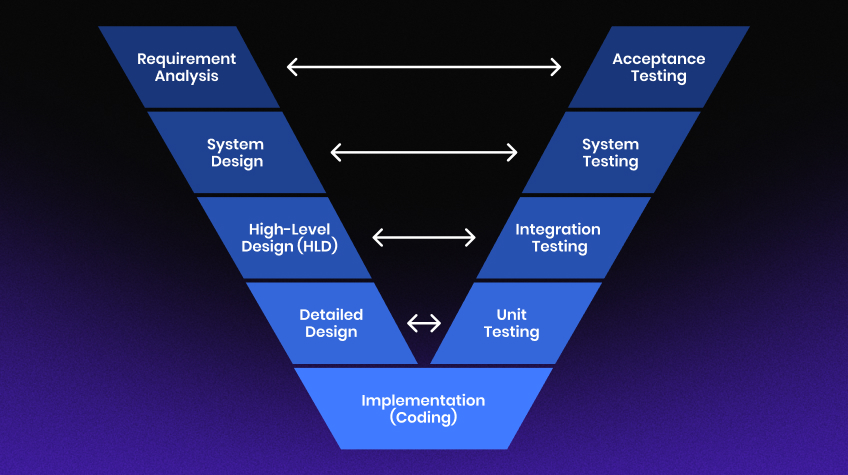
\includegraphics[width=0.85\textwidth]{logos/vmodel.jpg}
    \caption{V-Model methodology}
    \label{fig:v-model-methodology}
\end{figure}
\subsection{Software :Gantt Diagram}

% ── FIGURE: Gantt diagram (use StarUML or draw manually) ──
 \begin{figure}[H]
     \centering
     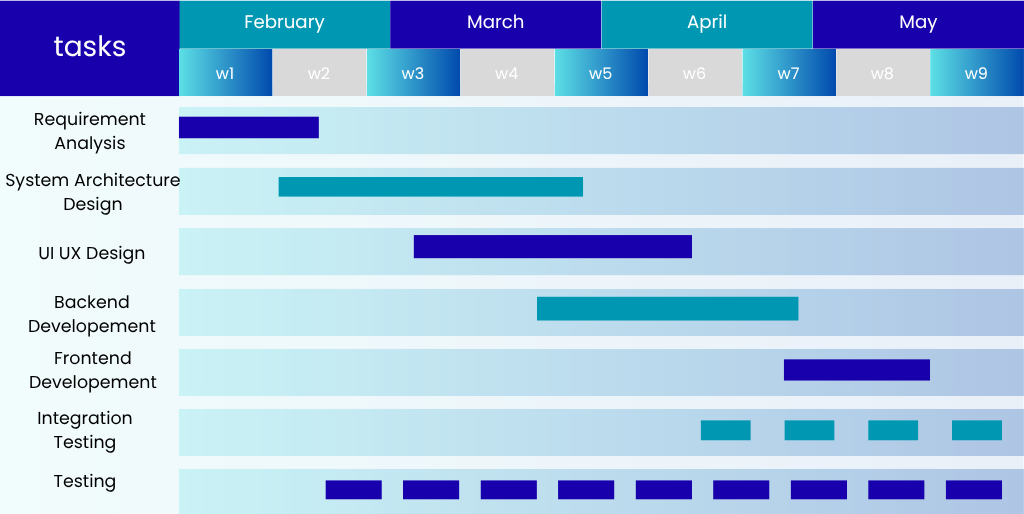
\includegraphics[width=\textwidth]{diagram/gant.png}
     \caption{Gantt diagram of the project}
     \label{fig:gantt}
 \end{figure}
\subsection{Artificial Intelligence: CRISP-DM Methodology } 
For the data science and AI modeling components, we strictly adhered to the \textbf{CRISP-DM} (Cross-Industry Standard Process for Data Mining) methodology. This industry-standard framework ensured our AI models remained focused on solving the core business problem. The six phases were implemented as follows:

\begin{enumerate}
    \item \textbf{Business Understanding:} We identified that content creators lack predictive insights before publishing. The objective was defined as building a Pre-Posting Predictive Agent to act as an algorithmic coach.
    \item \textbf{Data Understanding:} We collected over 1,100 short-form videos. Through Exploratory Data Analysis (EDA), we discovered the highly skewed power-law distribution of video views, which informed our mathematical approach.
    \item \textbf{Data Preparation:} We merged cross-platform metadata, sliced \texttt{.mp4} files into audio/visual components via FFmpeg, and applied Principal Component Analysis (PCA) to compress high-dimensional foundation model embeddings.
    \item \textbf{Modeling:} We trained and tuned multiple algorithms: XGBoost for tabular regression, \texttt{faster-whisper} for speech-to-text, and Real-ESRGAN/GFPGAN for Computer Vision upscaling.
    \item \textbf{Evaluation:} Models were rigorously tested using standard metrics (RMSE, $R^2$, PSNR). Crucially, evaluation led to the strategic decision to discard a noisy "Post-Posting" engagement model in favor of the highly accurate Pre-Posting agent.
    \item \textbf{Deployment:} The validated machine learning models were serialized and integrated into the Node.js Fastify backend, making them accessible to the end-user via the React interface.
\end{enumerate}
\subsection{Artificial Intelligence: Gantt Diagram}

% ── FIGURE: Gantt diagram (use StarUML or draw manually) ──
 \begin{figure}[H]
     \centering
     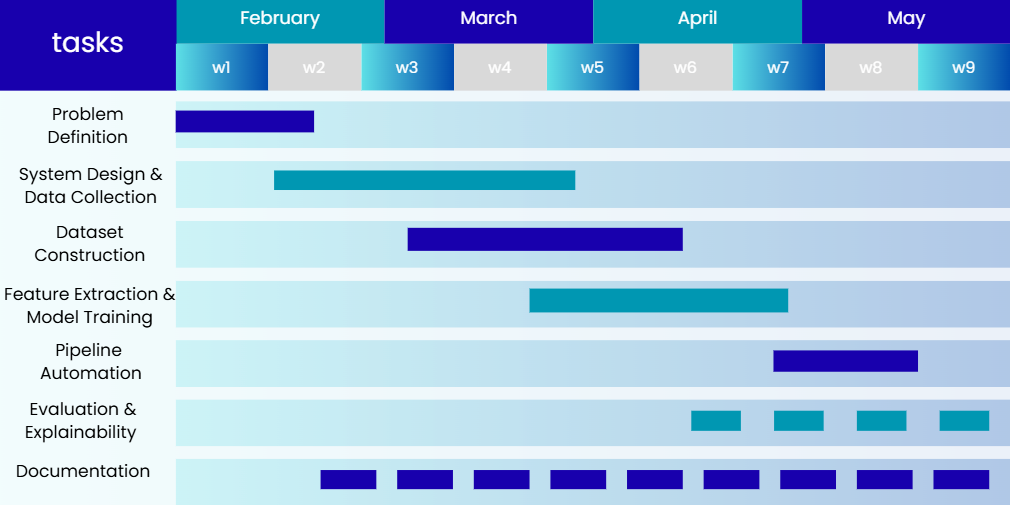
\includegraphics[width=\textwidth]{images/ganttAI.png}
     \caption{Gantt diagram of the AI part }
     \label{fig:gantt_AI}
 \end{figure}


\section*{Conclusion}
\phantomsection
\addcontentsline{toc}{section}{Conclusion}

In this chapter, we presented the general context of the \textbf{BViral Control Center} project and highlighted the growing challenges faced by content creators in managing and optimizing their presence across multiple social media platforms. Through the study and critical analysis of existing solutions such as Hootsuite, Buffer, and Topaz Video AI, we identified several limitations, particularly the lack of integration between social media management and AI-powered video enhancement.

To address these shortcomings, we proposed a unified and intelligent platform that combines scheduling, analytics, account management, AI video enhancement, and integrated video editing within a single ecosystem. We also introduced the theoretical foundations and state-of-the-art technologies adopted in our solution, including Machine Learning, Explainable AI, Computer Vision, and modern multimodal models.

Furthermore, we defined the functional and non-functional requirements of the system and presented the Agile iterative methodology selected for the project development. This methodology ensures flexibility, modularity, and continuous improvement throughout the implementation process.

The next chapter will focus on the system analysis and design phase, where we will present the global architecture, modeling diagrams, database design, and the technical structure of the proposed solution.
\chapter{Requirements Analysis and Data Specification}

\section*{Introduction}
\phantomsection
\addcontentsline{toc}{section}{Introduction}

\section{Requirements Modelling}

\subsection{Use-Case Diagram}
\subsubsection{Global Use Case Diagram}

The figure below presents the global use case diagram for the content creator, showing all major functionalities accessible from the dashboard.

% ── FIGURE: Global use case diagram ──
 \begin{figure}[H]
     \centering
     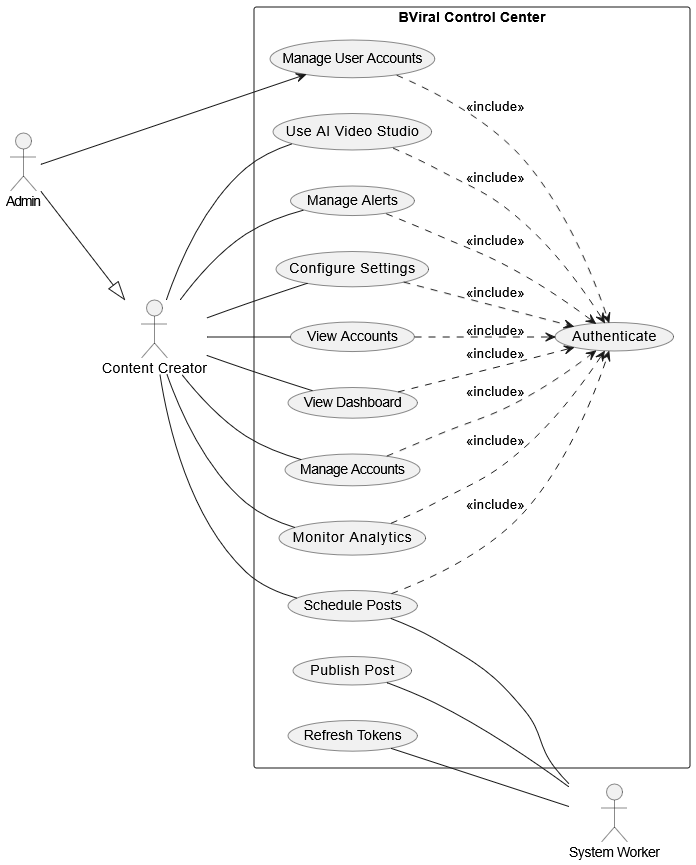
\includegraphics[width=0.65\textwidth]{diagram/diagram1.png}
     \caption{Global use case diagram for the Content Creator and admin}
     \label{fig:uc-global}
 \end{figure}

\vspace{0.5cm}

The content creator and admin interact with the following subsystems after authentication:
\begin{itemize}
    \item Dashboard overview (KPIs and statistics)
    \item Account management (connect/disconnect platforms)
    \item Post scheduling (create, view, cancel posts)
    \item Analytics monitoring
    \item AI Video Studio (enhance and edit videos)
    \item Alert management
    \item System settings
\end{itemize}

In addition, the admin has exclusive privileges for user management. Specifically, the admin is responsible for managing content creator accounts, including creating new accounts, updating user information, deleting accounts, and controlling access permissions. This ensures proper system governance, security, and centralized control over platform users.
%subsubsection*{Use Case Diagram: Account Management}

 \begin{figure}[H]
     \centering
     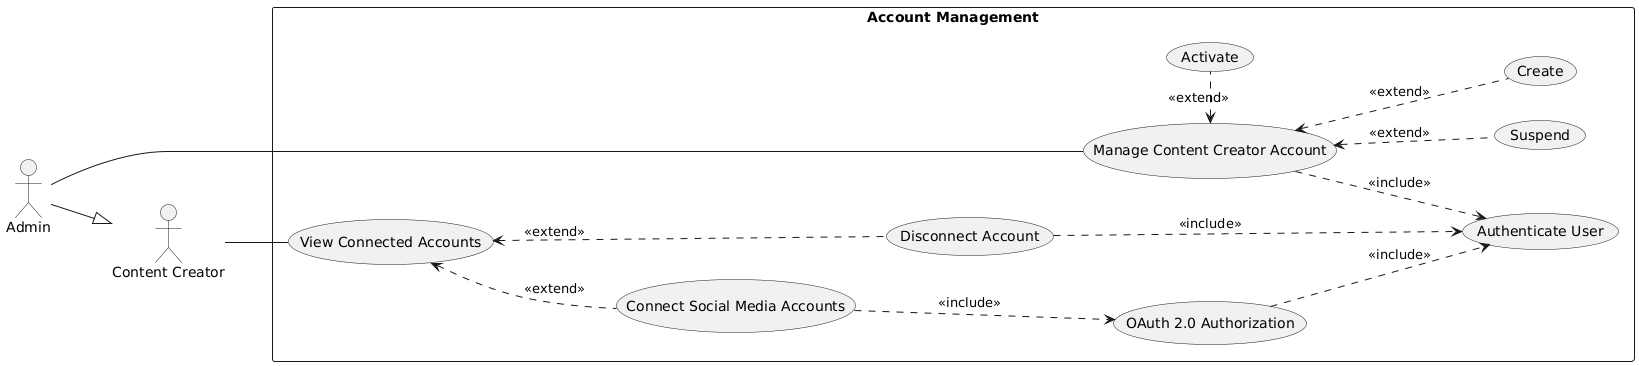
\includegraphics[width=0.95\textwidth]{diagram/diagram 2.png}
     \caption{Use case diagram of ``Account Management''}
     \label{fig:uc-accounts}
 \end{figure}

 \begin{table}[H]
\centering
\renewcommand{\arraystretch}{1.4}
\begin{tabular}{|p{4cm}|p{10cm}|}
\hline
\textbf{Title} & Account Management \\ \hline

\textbf{Actor} & Content Creator / Admin \\ \hline

\textbf{Summary} & 
This use case allows the actor to manage connected social media accounts and content creator accounts. \\ \hline

\textbf{Precondition} & 
The actor must be authenticated. \\ \hline

\textbf{Postcondition} & 
Accounts are successfully connected, modified, viewed, or deleted. \\ \hline

\textbf{Main Scenario} & 
- The actor accesses the account management module \newline
- The system displays the connected accounts \newline
- The actor can connect a new social media account \newline
- The system performs OAuth 2.0 authorization \newline
- The actor can view or disconnect an account \newline
- The admin can manage content creator accounts \newline
- The system saves the performed changes \\ \hline

\textbf{Alternative Scenario} & 
- Authentication failure \newline
- OAuth 2.0 authorization failure \newline
- Social media account already connected \newline
- Error while deleting or modifying an account \\ \hline

\end{tabular}
\caption{Use Case Description — Account Management}
\label{tab:account-management}
\end{table}

%\subsubsection*{Use Case Diagram: Post Scheduling}

 \begin{figure}[H]
     \centering
     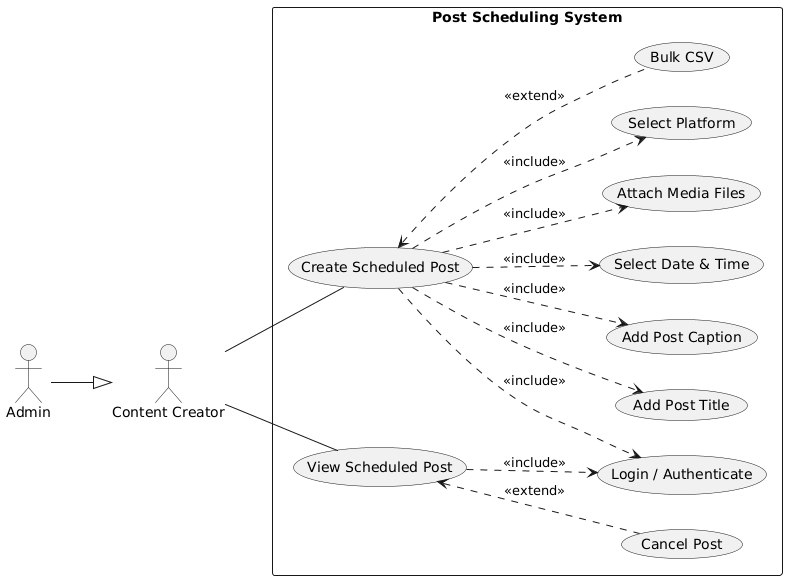
\includegraphics[width=0.75\textwidth]{diagram/diagram 3.png}
     \caption{Use case diagram of ``Post Scheduling''}
     \label{fig:uc-analytics}
 \end{figure}

%\noindent\textit{See StarUML code --- Diagram 3.}

\begin{table}[H]
\centering
\renewcommand{\arraystretch}{1.4}
\begin{tabular}{|p{4cm}|p{10cm}|}
\hline
\textbf{Title} & Post Scheduling System \\ \hline

\textbf{Actor} & Content Creator / Admin \\ \hline

\textbf{Summary} & 
This use case allows the actor to create, schedule, view, and cancel social media posts. \\ \hline

\textbf{Precondition} & 
The actor must be authenticated. \\ \hline

\textbf{Postcondition} & 
The post is successfully scheduled, viewed, or canceled. \\ \hline

\textbf{Main Scenario} & 
- The actor accesses the post scheduling module \newline
- The actor must authenticate \newline
- The actor creates a scheduled post \newline
- The actor must add post title\newline
- The actor must add post caption\newline
- The actor must select the target platform \newline
- The actor must select the publication date and time \newline
- The actor must attache media files \newline
- The actor must save the scheduled post \newline
- The actor can view scheduled posts \newline
-The System Worker actor automatically publishes posts at their scheduled time
using BullMQ queues\newline
- The actor can Bulk CSV \\ \hline

\textbf{Alternative Scenario} & 
- Authentication failure \newline
- Invalid publication date or time \newline
- Unsupported media file format \newline
- Failure while uploading media files \newline
- Error while canceling the scheduled post \newline
- Bulk CSV import contains invalid data \\ \hline

\end{tabular}
\caption{Use Case Description — Post Scheduling System}
\label{tab:post-scheduling-system}
\end{table}


%\noindent\textit{See StarUML code --- Diagram 5.}
\subsubsection*{Use Case Diagram: Use Ai studio}
 \begin{figure}[H]
     \centering
     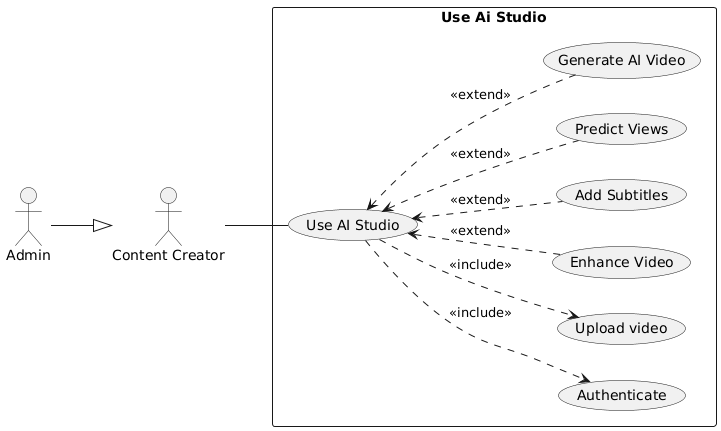
\includegraphics[width=0.65\textwidth]{diagram/diagram 5.png}
     \caption{Use case diagram of ``Alert Management''}
     \label{fig:uc-alerts}
 \end{figure}

\begin{table}[H]
\centering
\renewcommand{\arraystretch}{1.4}
\begin{tabular}{|p{4cm}|p{10cm}|}
\hline
\textbf{Title} & Use AI Studio \\ \hline

\textbf{Actor} & Content Creator / Admin \\ \hline

\textbf{Summary} & 
This use case allows the actor to access and use the AI Studio platform where they can upload videos, enhance content, generate AI videos, add subtitles, and predict video performance. \\ \hline

\textbf{Precondition} & 
The actor must be authenticated. \\ \hline

\textbf{Postcondition} & 
The actor successfully uses AI Studio features such as upload, enhancement, generation, and analytics. \\ \hline

\textbf{Main Scenario} & 
- The user accesses the AI Studio dashboard \newline
- The system authenticates the actor \newline
- The user must upload a video \newline
- The user can select an AI feature (enhance, subtitles, prediction, or generation) \\ \hline

\textbf{Alternative Scenario} & 
- Authentication failure \newline
- Upload failure due to unsupported format \newline
- AI processing error or timeout \newline
- Insufficient system resources for video generation \newline
- Invalid input parameters for AI processing \\ \hline

\end{tabular}
\caption{Use Case Description — Use AI Studio}
\label{tab:use-ai-studio}
\end{table}

\subsubsection*{Use Case Diagram: Admin Management}

In addition to the use cases shared with content creators, the administrator interacts with a dedicated set of supervisory features. These features were progressively added during the project (database migration \texttt{0006\_admin\_overhaul.sql}) to give the platform a real governance layer rather than a flat multi-tenant model.

\begin{table}[H]
\centering
\renewcommand{\arraystretch}{1.4}
\begin{tabular}{|p{4cm}|p{10cm}|}
\hline
\textbf{Title} & Admin Management \\ \hline

\textbf{Actor} & Admin \\ \hline

\textbf{Summary} &
This use case groups every administrator-only capability: governance of content creator accounts, oversight of all posts and videos across the platform, global analytics, soft-delete recovery (Trash), audit trail consultation, and operational monitoring of the job queues. \\ \hline

\textbf{Precondition} &
The actor must be authenticated and the resolved role from the Supabase JWT (claim \texttt{app\_role}) or the local user table must equal \texttt{admin}. \\ \hline

\textbf{Postcondition} &
The administrative action is executed, persisted, and a corresponding entry is written to the immutable admin audit log. \\ \hline

\textbf{Main Scenario} &
- The admin accesses the dedicated \texttt{/admin/*} routes through the dashboard sidebar \newline
- The backend re-checks the admin role via the \texttt{requireRole("admin")} Fastify decorator on every protected endpoint \newline
- The admin invites, edits, suspends, or removes a content creator from the Creators page \newline
- The admin browses every scheduled post or uploaded video across the whole platform (cross-tenant view) \newline
- The admin consults Global Analytics with filters, time ranges, and CSV export \newline
- The admin restores or permanently removes soft-deleted posts from the Trash page \newline
- The admin reviews the immutable audit trail of every administrative write \newline
- The admin monitors queue depth, failed jobs, and triggers one-click retries on the System Health page \newline
- The system records each write action into the \texttt{admin\_audit\_log} table \\ \hline

\textbf{Alternative Scenario} &
- The user is authenticated but does not hold the admin role: the API returns 403 Forbidden \newline
- The targeted account is already suspended or already deleted \newline
- A retried job ID no longer exists in the queue \newline
- The audit-log write fails (the original operation is still committed, but a warning is logged) \\ \hline

\end{tabular}
\caption{Use Case Description --- Admin Management}
\label{tab:admin-management}
\end{table}

\subsubsection*{Use Case Diagram: System Monitoring}

Beyond business-level oversight, the administrator also supervises the operational health of the platform. This use case formalises the System Health view and the retry workflow.

\begin{table}[H]
\centering
\renewcommand{\arraystretch}{1.4}
\begin{tabular}{|p{4cm}|p{10cm}|}
\hline
\textbf{Title} & System Monitoring \\ \hline

\textbf{Actor} & Admin \\ \hline

\textbf{Summary} &
This use case allows the administrator to inspect the runtime state of the four BullMQ queues (post-publishing, video-processing, analytics-refresh, ai-processing), browse failed jobs, and trigger a manual retry. \\ \hline

\textbf{Precondition} &
The actor must be authenticated as admin. Redis must be reachable and the API must be running. \\ \hline

\textbf{Postcondition} &
The selected job is re-enqueued. The retry action is recorded in the admin audit log under the \texttt{system.retry\_job} action. \\ \hline

\textbf{Main Scenario} &
- The admin opens the System Health page \newline
- The dashboard calls \texttt{GET /api/v1/admin/system/health} which aggregates job counts (waiting, active, completed, failed, delayed, paused) for each queue \newline
- The admin selects a queue and lists its failed jobs via \texttt{GET /api/v1/admin/system/failed-jobs?queue=...} \newline
- The admin clicks ``retry'' on a specific job, triggering \texttt{POST /system/jobs/:queue/:jobId/retry} \newline
- The system writes an audit entry and returns the new job state \\ \hline

\textbf{Alternative Scenario} &
- The queue name is invalid (validation error from the Zod schema) \newline
- The job ID no longer exists (404 Not Found) \newline
- Redis is unreachable (the System Health card displays a degraded state) \\ \hline

\end{tabular}
\caption{Use Case Description --- System Monitoring}
\label{tab:system-monitoring}
\end{table}

\subsection{Class Diagram}
The class diagram represents the data model of BViral Control Center. The main entities and their relationships are:

%\noindent\textit{See StarUML code --- Diagram 7 (Class Diagram).}

 \begin{figure}[H]
     \centering
     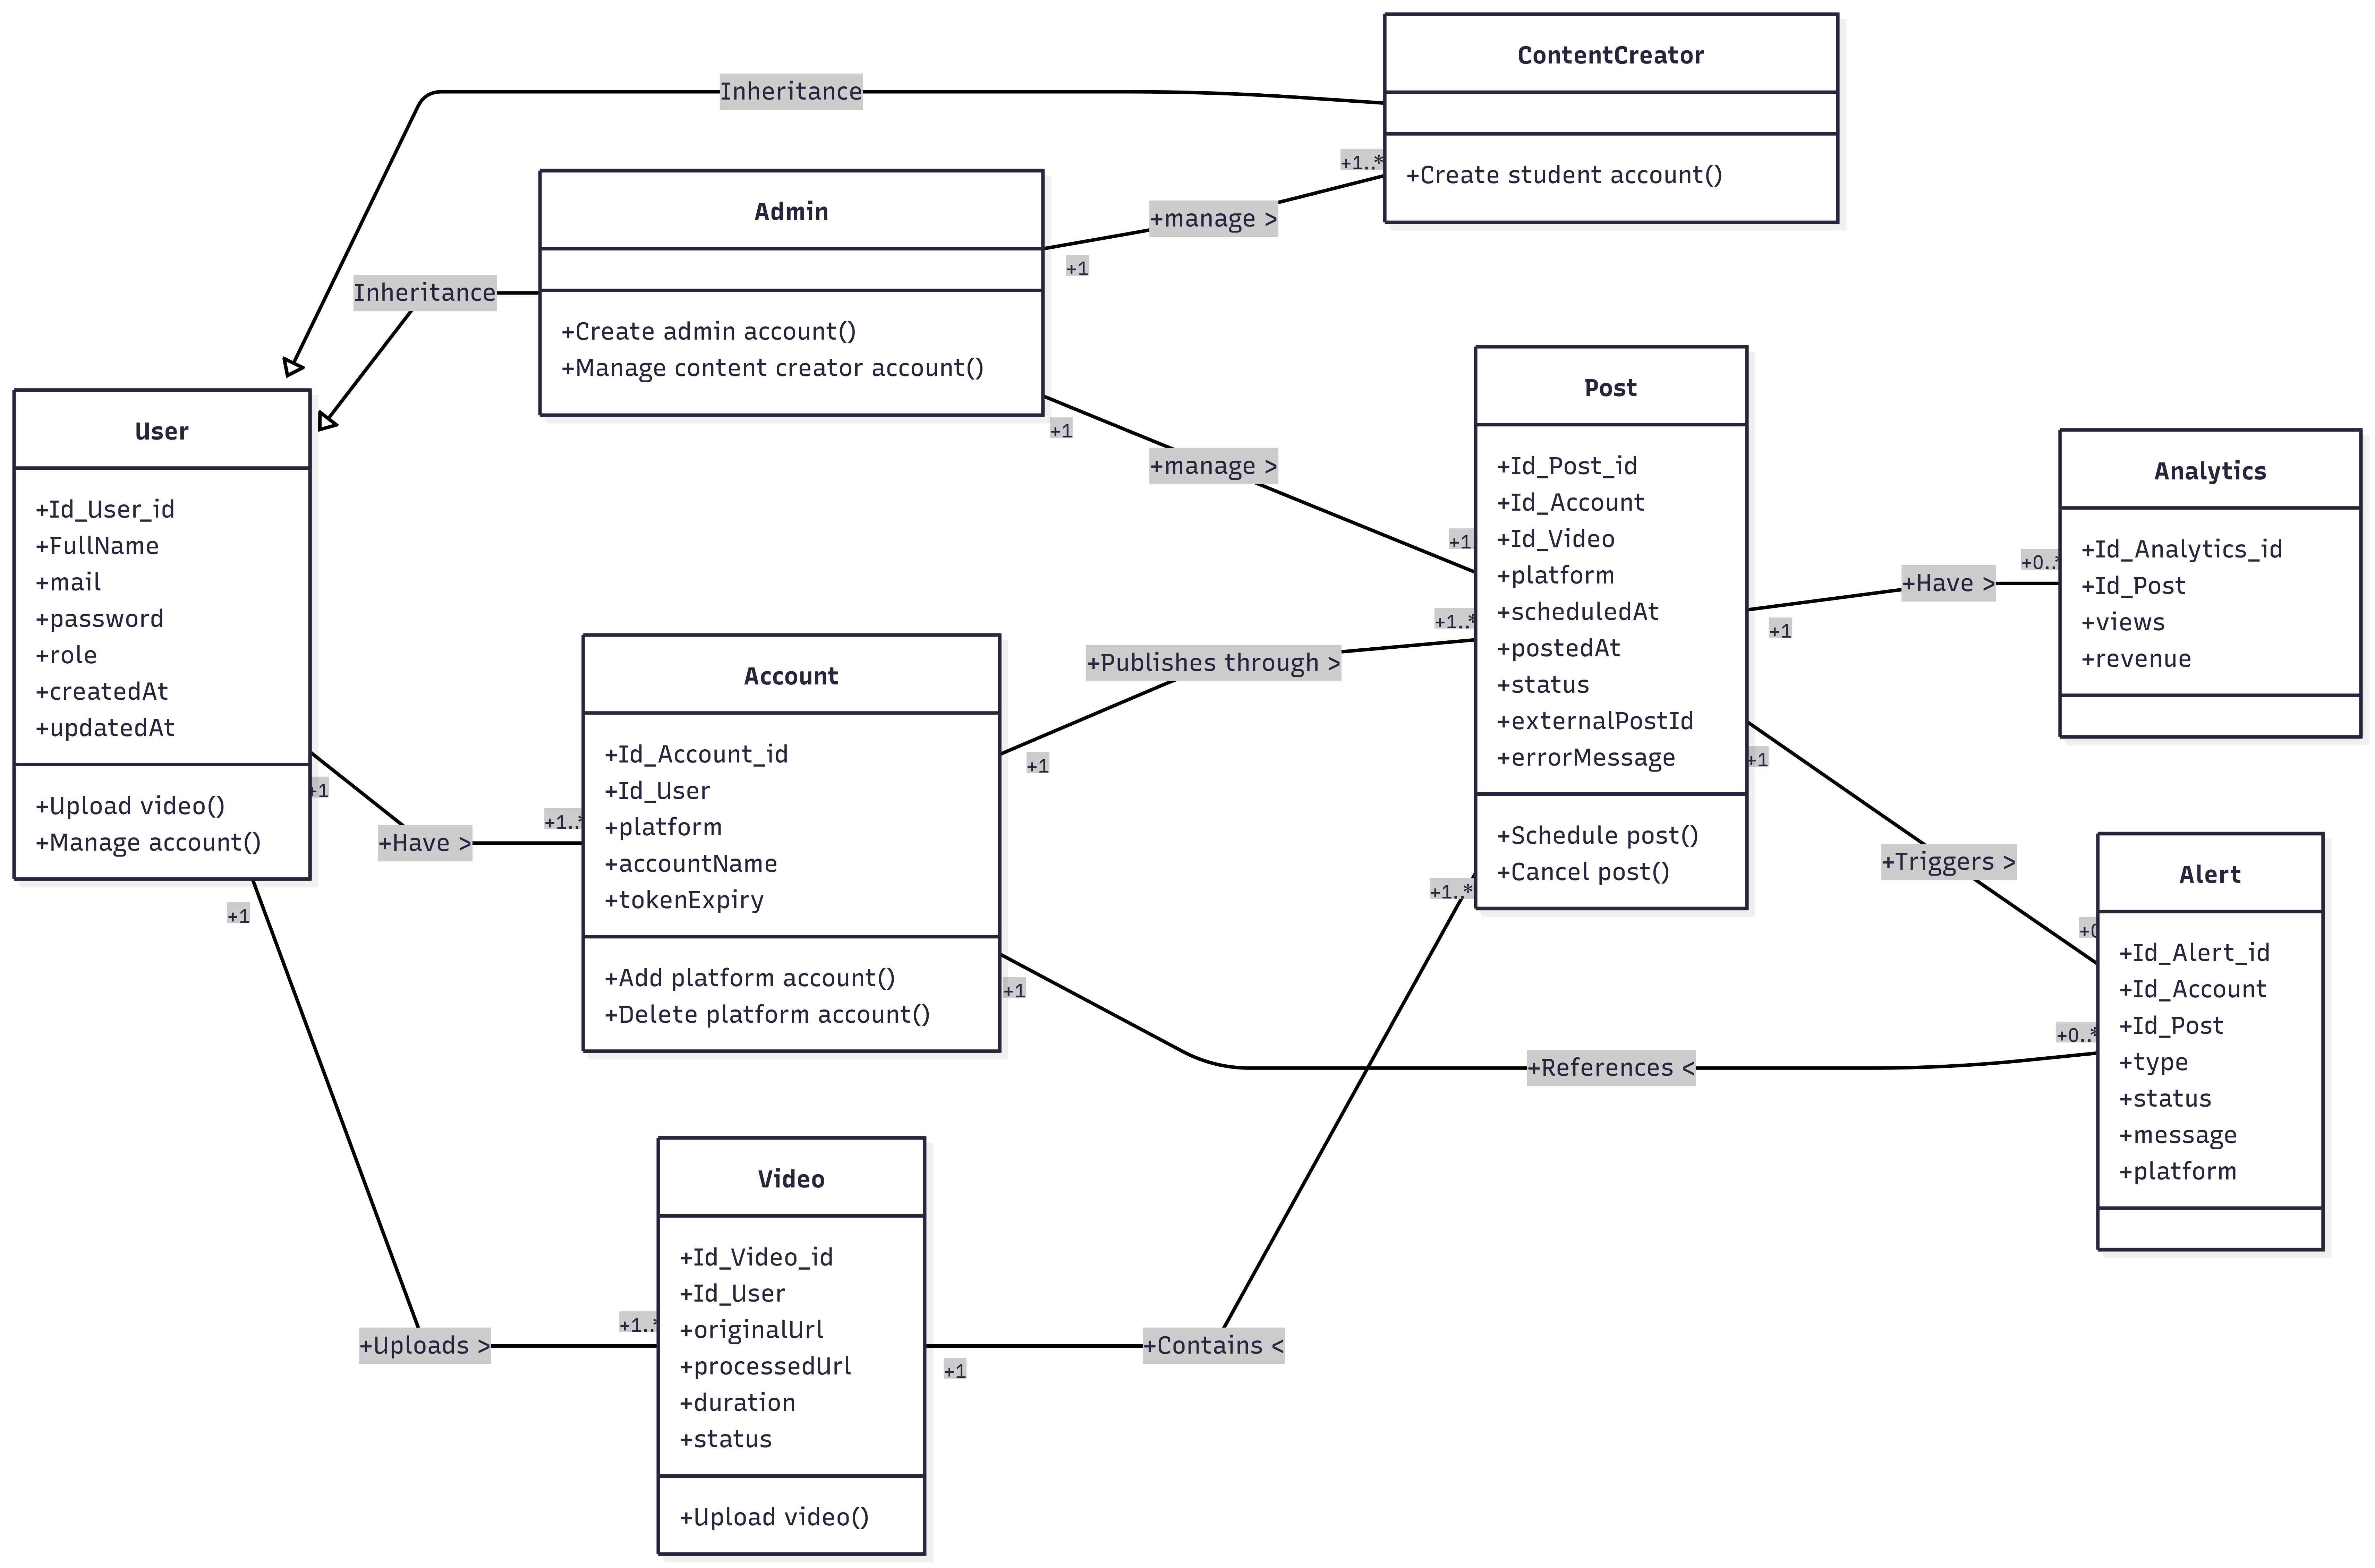
\includegraphics[width=\textwidth]{diagram/diagram class.png}
     \caption{Class diagram of BViral Control Center}
     \label{fig:class-diagram}
 \end{figure}

The system contains six main entities:
\begin{itemize}
    \item \textbf{User:} Represents a registered system user with attributes: \textit{Id\_User}, \textit{FullName}, \textit{mail}, \textit{password}, \textit{role}, \textit{createdAt}, and \textit{updatedAt}. It offers functionalities to \textit{Upload video()} and \textit{Manage account()}. It serves as the base class for two specialized roles:
    \begin{itemize}
        \item \textbf{ContentCreator:} Inherits from User and provides the capability to \textit{Create student account()}.
        \item \textbf{Admin:} Inherits from User and provides capabilities to \textit{Create admin account()} and \textit{Manage content creator account()}.
    \end{itemize}
    \item \textbf{Account:} Represents a linked platform account connected to a User, with attributes: \textit{Id\_Account\_id}, \textit{Id\_User}, \textit{platform}, \textit{accountName}, and \textit{tokenExpiry}. It handles functionalities to \textit{Add platform account()} and \textit{Delete platform account()}.
    \item \textbf{Video:} Represents a video asset uploaded by a User, with attributes: \textit{Id\_Video\_id}, \textit{Id\_User}, \textit{originalUrl}, \textit{processedUrl}, \textit{duration}, and \textit{status}. It includes an \textit{Upload video()} method.
    \item \textbf{Post:} Represents a scheduled or published publication linked to an Account and a Video, with attributes: \textit{Id\_Post\_id}, \textit{Id\_Account}, \textit{Id\_Video}, \textit{platform}, \textit{scheduledAt}, \textit{postedAt}, \textit{status}, \textit{externalPostId}, and \textit{errorMessage}. It handles functionalities to \textit{Schedule post()} and \textit{Cancel post()}.
    \item \textbf{Analytics:} Stores performance metrics linked to a specific Post, tracking: \textit{Id\_Analytics\_id}, \textit{Id\_Post}, \textit{views}, and \textit{revenue}.
    \item \textbf{Alert:} Represents system notifications triggered by posts or referenced by accounts, with attributes: \textit{Id\_Alert\_id}, \textit{Id\_Account}, \textit{Id\_Post}, \textit{type}, \textit{status}, \textit{message}, and \textit{platform}.
    \item \textbf{AdminAuditLog:} Immutable trace of every administrative write action, with attributes: \textit{Id\_AuditLog}, \textit{Id\_Admin}, \textit{action} (e.g.\ \texttt{system.retry\_job}, \texttt{creator.suspend}, \texttt{post.soft\_delete}), \textit{targetType}, \textit{targetId}, \textit{payload} (JSONB), and \textit{createdAt}. The table is indexed on \texttt{(adminId, createdAt)} and \texttt{(targetType, targetId)} for fast forensic queries.
\end{itemize}

\medskip
\noindent\textbf{Additional persistence-level attributes worth noting:}
\begin{itemize}
    \item The \textit{User} entity carries \textit{role} (\texttt{admin} or \texttt{content\_creator}), \textit{suspendedAt}, and \textit{suspendedBy} to support administrative governance.
    \item The \textit{Post} entity carries \textit{deletedAt} and \textit{deletedBy} to implement \emph{soft-delete} and the Trash recovery workflow.
    \item The \textit{Video} entity carries a \textit{contentHash} (SHA indexed on \texttt{(userId, contentHash)}) used to detect duplicate uploads.
    \item The \textit{Account} entity stores OAuth credentials (\textit{accessToken}, \textit{refreshToken}, \textit{tokenExpiry}). Tokens are persisted encrypted at rest using AES-256-GCM (see Chapter~3).
\end{itemize}


\textbf{Relationships:}
\begin{itemize}
    \item User $\xrightarrow{1..*}$ Account (a user owns multiple accounts)
    \item User $\xrightarrow{1..*}$ Video (a user uploads multiple videos)
    \item Account $\xrightarrow{1..*}$ Post (posts are published through accounts)
    \item Video $\xrightarrow{1..*}$ Post (a video can be posted to multiple platforms)
    \item Post $\xrightarrow{0..*}$ Analytics (each post has analytics snapshots)
    \item Account $\xrightarrow{0..*}$ Alert (alerts may reference an account)
    \item Post $\xrightarrow{0..*}$ Alert (alerts may reference a post)
\end{itemize}


\subsection{Sequence Diagrams}



\subsubsection{Sequence Diagram: Authentification}
%\noindent\textit{See StarUML code --- Diagram 8.}

 \begin{figure}[H]
     \centering
     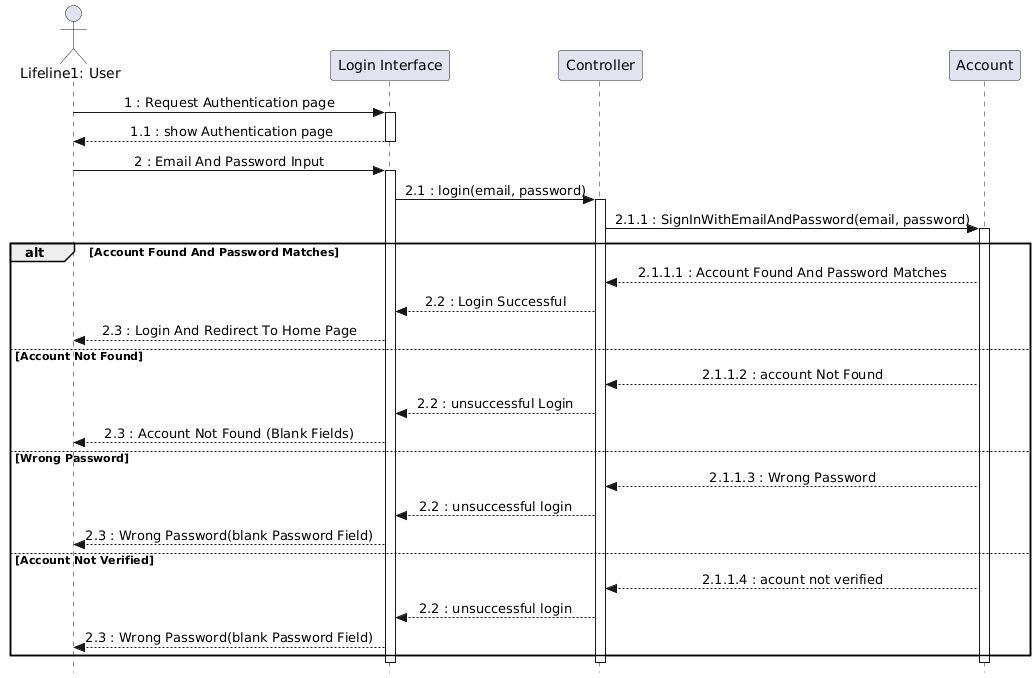
\includegraphics[width=\textwidth]{diagram/diagramme sequence 1.png}
     \caption{Sequence diagram of Authentification}
     \label{fig:seq-oauth}
 \end{figure}

\begin{enumerate}
    \item The user requests the authentication page via the login interface to access the application dashboard.
    \item The user inputs their credentials, specifying their email and password, into the login form.
    \item The login interface transmits the credentials to the backend application layer by invoking the login handler.
    \item The controller authenticates the submission details by requesting a lookup from the core account management service.
    \item The account service verifies the credentials against the identity database, checking for user existence, password matches, and verification flags.
    \item On success, the account confirmation is returned to the interface, which authenticates the session and redirects the user to the application home page.
    \item On validation failure (such as account not found, incorrect password, or unverified profile status), an unsuccessful login status is returned, displaying a precise error message to the interface.
\end{enumerate}

\subsubsection{Sequence Diagram: Post Scheduling}
%\noindent\textit{See StarUML code --- Diagram 9.}

 \begin{figure}[H]
     \centering
     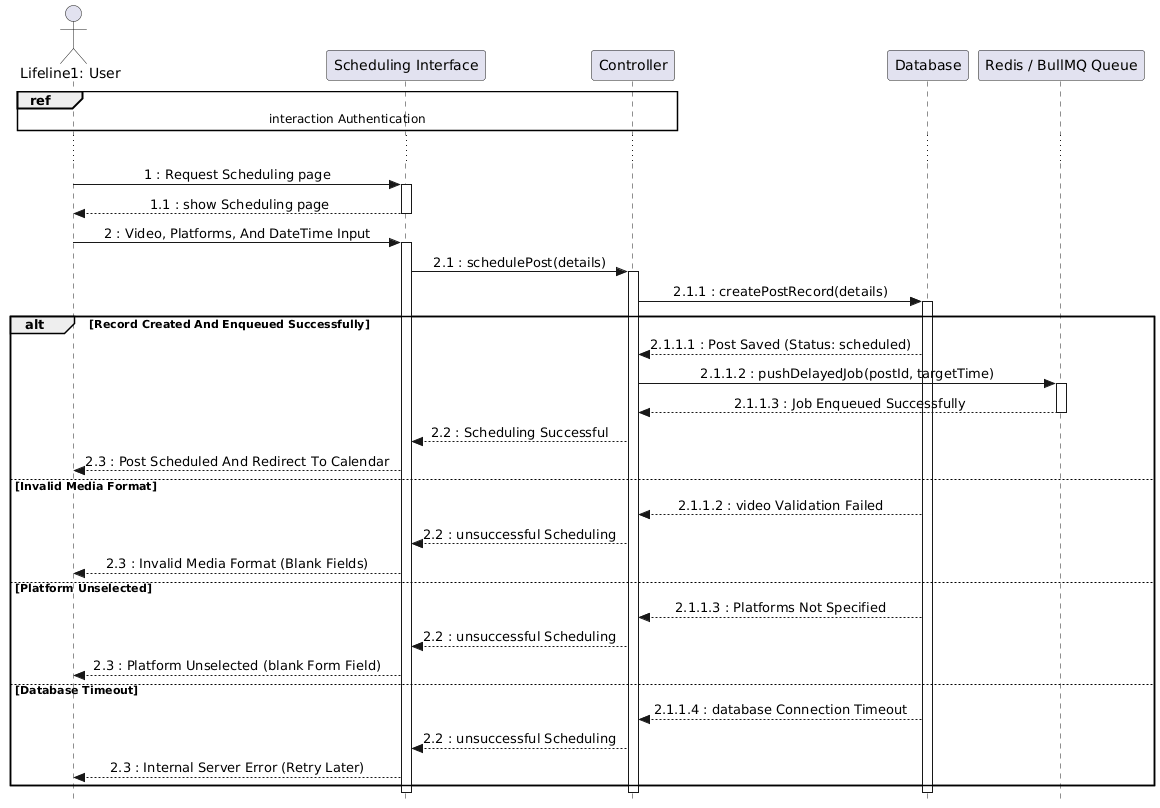
\includegraphics[width=\textwidth]{diagram/diagramme sequence 2.png}
     \caption{Sequence diagram of ``Schedule and Publish a Post''}
     \label{fig:seq-schedule}
 \end{figure}

The scheduling and publishing flow:
\begin{enumerate}
    \item The user creates a new post in the scheduling interface, selecting video, platform, account, and schedule time.
    \item The dashboard sends a POST request to \texttt{/api/v1/posts}.
    \item The API server validates the request, creates a post record with status ``scheduled'', and enqueues a delayed job in the Redis/BullMQ publishing queue.
    \item At the scheduled time, the BullMQ worker dequeues the job.
    \item The worker calls the appropriate platform publisher service (YouTube, TikTok, or Meta).
    \item The platform service uploads the video and metadata using the stored OAuth tokens.
    \item On success, the post status is updated to ``posted'' with the external post ID. On failure, it is marked ``failed'' with an error message, and an alert is created.
\end{enumerate}

\section{AI Pipeline Specification \& Processing Steps}

The analytical method follows a strict end-to-end Machine Learning pipeline, summarized in Figure~\ref{fig:ai-workflow-diagram}.

\begin{figure}[H]
    \centering
    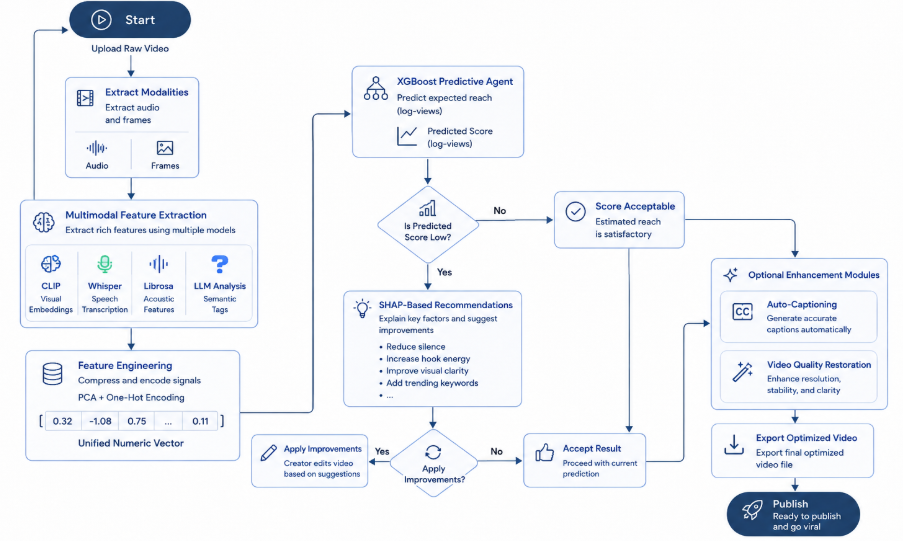
\includegraphics[width=0.9\textwidth]{images/0workflowdiagram.png}
    \caption{Workflow diagram of the AI pipeline and processing steps}
    \label{fig:ai-workflow-diagram}
\end{figure}
\begin{enumerate}
    \item \textbf{Data Ingestion:} Raw \texttt{.mp4} videos are uploaded and split into audio (\texttt{.wav}) and video frames using \texttt{FFmpeg}.
    \item \textbf{Feature Extraction \& Preprocessing:} Multimodal foundation models (CLIP, Librosa, Whisper, Llama 3) extract high-dimensional semantic data.
    \item \textbf{Feature Engineering:} Principal Component Analysis (PCA) compresses the dense vectors (e.g., 512D to 64D) to prevent overfitting. Categorical LLM tags are One-Hot Encoded.
    \item \textbf{Model Training:} The final 473-dimensional vector is fed into the XGBoost Regressor to map content features to the \texttt{log\_views} target.
    \item \textbf{Evaluation \& XAI:} The model is evaluated using RMSE and $R^2$. SHAP (SHapley Additive exPlanations) is applied to extract actionable feedback.
    \item \textbf{Deployment:} The trained model, scalers, and PCA transformers are exported via \texttt{pickle} for integration into the final application.
\end{enumerate}



\section*{Conclusion}
\phantomsection
\addcontentsline{toc}{section}{Conclusion}
In this chapter, we analyzed and modeled the functional and structural requirements of the BViral Control Center platform. Use-case diagrams and detailed scenarios were used to describe the interactions between users and the system, while the class diagram defined the main entities and their relationships. Sequence diagrams illustrated the dynamic behavior of key processes such as authentication and post scheduling. Finally, the AI pipeline specification presented the workflow of the intelligent video processing and prediction system. These analyses provide a solid foundation for the implementation phase discussed in the next chapter.
\chapter{System Design and Realisation}


\section*{Introduction}
In this chapter, we focus on the technical realization of BViral Control Center. We present the system architecture, justify our technology choices, describe the development environment and tools, and showcase the implemented interfaces through screenshots.

% ══════════════════════════════════════════════════════════════
\section{System Architecture}
% ══════════════════════════════════════════════════════════════
This section describes the overall system architecture of the BViral Control Center platform. It presents the structural organization of the system, highlighting how the different components are distributed across the monorepo workspace, how they interact within a client-server model, and how the backend is structured following an MVC-inspired pattern. This architectural design ensures modularity, scalability, and clear separation of concerns across all system layers.
\subsection{Monorepo Workspace Architecture}

BViral Control Center is organized as a \textbf{pnpm monorepo workspace}, a modern approach that allows multiple packages (frontend, backend, shared libraries) to coexist in a single repository while maintaining clear separation of concerns.

% \begin{figure}[H]
%     \centering
%     \includegraphics[width=0.85\textwidth]{figures/arch_monorepo.png}
%     \caption{pnpm Monorepo workspace architecture}
%     \label{fig:arch-monorepo}
% \end{figure}

The workspace is divided into three layers:

\begin{itemize}
    \item \textbf{artifacts/} --- Deployable applications:
    \begin{itemize}
        \item \texttt{bviral-dashboard}: React/Vite frontend dashboard
        \item \texttt{api-server}: Fastify REST API backend
        \item \texttt{openvideo}: Vendored BVIRAL Video Editor (Next.js)
        \item \texttt{mockup-sandbox}: UI prototyping sandbox
    \end{itemize}
    \item \textbf{lib/} --- Shared packages:
    \begin{itemize}
        \item \texttt{db}: Drizzle ORM schema and database helpers
        \item \texttt{api-spec}: OpenAPI specification and codegen config
        \item \texttt{api-zod}: Generated Zod validation schemas
        \item \texttt{api-client-react}: Generated React API client
    \end{itemize}
    \item \textbf{scripts/} --- Utility and automation scripts
\end{itemize}

\subsection{Client-Server Architecture}

The system follows a classic \textbf{client-server architecture} with clear separation between the presentation layer and the business/data layers.

% \begin{figure}[H]
%     \centering
%     \includegraphics[width=0.9\textwidth]{figures/arch_client_server.png}
%     \caption{Client-Server architecture of BViral}
%     \label{fig:arch-cs}
% \end{figure}

\begin{itemize}
    \item \textbf{Presentation Tier (Client):} The React/Vite dashboard served at \texttt{localhost:5173}. It communicates with the API via RESTful HTTP requests and renders the UI using React components, Tailwind CSS, and Framer Motion.
    \item \textbf{Business Logic Tier (API Server):} The Fastify server at \texttt{localhost:3001} handles authentication, OAuth flows, CRUD operations, and orchestrates the BullMQ post-publishing worker.
    \item \textbf{Data Tier:} PostgreSQL database (hosted via Supabase) managed through Drizzle ORM with type-safe schemas and Row Level Security (RLS) policies. Redis is used for BullMQ job queues.
    \item \textbf{AI Processing Tier:} Python-based AI video enhancement pipeline using PyTorch, Real-ESRGAN, GFPGAN, and OpenCV, running independently or integrated via API calls.
\end{itemize}

\subsection{MVC-Inspired Pattern}

The API server follows an MVC-inspired layered architecture:

\begin{itemize}
    \item \textbf{Routes (Controller):} Define HTTP endpoints, handle request validation, and delegate to services. Organized under \texttt{/api/v1/} with sub-routers for accounts, posts, videos, analytics, alerts, and users.
    \item \textbf{Services (Business Logic):} Contain the core business logic for each domain. Services include \texttt{accounts.service}, \texttt{posts.service}, \texttt{analytics.service}, \texttt{youtube.service}, \texttt{tiktok.service}, \texttt{meta.service}, \texttt{videos.service}, \texttt{alerts.service}, and \texttt{platform-publisher.service}.
    \item \textbf{Schema/Repository (Model):} Drizzle ORM schemas define the database structure. Repositories provide data access methods with type-safe queries.
\end{itemize}

\subsection{Fastify Plugin Architecture}

The API server is built on top of Fastify's plugin system. Plugins are auto-loaded from \texttt{src/plugins/} in a strict, numbered order so that each plugin can safely depend on the ones registered before it:

\begin{itemize}
    \item \texttt{00-config} --- environment loading and configuration parsing.
    \item \texttt{10-observability} --- structured request/response logging with request-id correlation.
    \item \texttt{20-cors} --- CORS allow-list from \texttt{CORS\_ORIGINS}.
    \item \texttt{25-multipart} --- multipart parser for video uploads.
    \item \texttt{30-database} --- PostgreSQL connection pool (configurable \texttt{dbPoolMax}) and the Drizzle instance.
    \item \texttt{35-storage} --- Supabase service-role client for privileged storage operations.
    \item \texttt{38-queues} --- BullMQ queue accessors (post-publishing, video-processing, analytics-refresh, ai-processing) and the \texttt{queuesAdmin} decorator used by the System Health page.
    \item \texttt{40-repositories} --- dependency-injected repositories (accounts, posts, videos, analytics, alerts, users, admin-posts, admin-videos, admin-audit).
    \item \texttt{45-ai} --- AI processing pipeline wiring (LTX, captioning, enhancement).
    \item \texttt{50-auth} --- Supabase JWT verification, role resolution, suspension check, and the \texttt{authenticate} / \texttt{requireRole} decorators.
\end{itemize}

Every domain route (\texttt{/api/v1/posts}, \texttt{/api/v1/accounts}, \texttt{/api/v1/admin/*}, \ldots) is itself loaded by \texttt{@fastify/autoload}, which keeps the route tree mechanically consistent with the directory layout.

% ══════════════════════════════════════════════════════════════
\section{Technology Choices}
% ══════════════════════════════════════════════════════════════
This section presents the main technologies used in the development of the BViral Control Center platform. The chosen stack was selected to ensure high performance, scalability, and maintainability across both frontend and backend layers, while also supporting real-time processing, AI integration, and efficient data management. Each technology plays a specific role within the system architecture, contributing to the overall functionality of the application.
\subsection{React \& Vite (Frontend)}

 \begin{figure}[H]
     \centering
     
\includegraphics[width=0.25\textwidth]{logos/react.png}
     \caption{React Frontend Framework}
     \label{fig:react}
 \end{figure}

  \begin{figure}[H]
     \centering
     
\includegraphics[width=0.25\textwidth]{logos/vite.png}
     \caption{Vite}
     \label{fig:react}
 \end{figure}

React 19 is a declarative, component-based JavaScript library for building user interfaces, maintained by Meta. Combined with Vite 7, a next-generation build tool, it provides near-instant hot module replacement (HMR) during development and optimized production builds. Key frontend libraries include:

\begin{itemize}
    \item \textbf{Tailwind CSS 4:} utility-first CSS framework for rapid, consistent styling.
    \item \textbf{Framer Motion:} production-ready animation library for React.
    \item \textbf{Wouter:} lightweight client-side router.
    \item \textbf{TanStack React Query:} data fetching and server-state management.
    \item \textbf{Lucide React:} modern, customizable icon library.
    \item \textbf{Recharts:} composable charting library for analytics visualization.
\end{itemize}

\subsection{Fastify (Backend)}

Fastify is a high-performance, low-overhead Node.js web framework. It is designed for speed and developer experience, featuring:

\begin{itemize}
    \item Schema-based request/response validation with AJV.
    \item Plugin-based architecture with auto-loading.
    \item Built-in logging via Pino with production-grade redaction.
    \item Native TypeScript support.
\end{itemize}

\begin{figure}[H]
    \centering
    
\includegraphics[width=0.25\textwidth]{logos/fastify.png}
    \caption{Fastify backend framework}
    \label{fig:fastify-logo}
\end{figure}

\subsection{PostgreSQL \& Drizzle ORM (Database)}

PostgreSQL is a powerful, open-source relational database system. We use Supabase as a hosted PostgreSQL provider, which adds built-in authentication and Row Level Security.

Drizzle ORM provides a type-safe, SQL-like query builder for TypeScript with:

\begin{itemize}
    \item Schema-as-code with full TypeScript type inference.
    \item Built-in Supabase RLS policy support.
    \item Zero-dependency, lightweight runtime.
    \item Push-based migration for schema changes.
\end{itemize}

\begin{figure}[H]
    \centering
    
\includegraphics[width=0.35\textwidth]{logos/postgre.png}
    \caption{Database PostgreSQL}
    \label{fig:PostgreSQL}
\end{figure}

\begin{figure}[H]
    \centering
    
\includegraphics[width=0.35\textwidth]{logos/supabase.png}
    \caption{Supabase database platform}
    \label{fig:supabase-logo}
\end{figure}

\begin{figure}[H]
    \centering
    
\includegraphics[width=0.35\textwidth]{drizzle.png}
    \caption{Drizzle ORM}
    \label{fig:drizzle-logo}
\end{figure}

\subsection{Redis \& BullMQ (Job Queue)}

Redis is used as the backing store for BullMQ, a robust Node.js job queue for managing scheduled post publishing. The worker restores pending jobs on restart and processes posts at their scheduled time, calling the appropriate platform API.

\begin{figure}[H]
    \centering
    
\includegraphics[width=0.3\textwidth]{logos/redis.png}
    \caption{Redis}
    \label{fig:Redis}
\end{figure}

\subsection{PyTorch, Real-ESRGAN \& GFPGAN (AI Pipeline)}

The AI video enhancement pipeline leverages:

\begin{itemize}
    \item \textbf{PyTorch:} deep learning framework with GPU and parallel CPU support.
    \item \textbf{Real-ESRGAN:} state-of-the-art super-resolution model for upscaling video frames (2x or 4x).
    \item \textbf{GFPGAN:} face restoration model that enhances facial details in video frames.
    \item \textbf{OpenCV:} computer vision library for classical filter processing (bilateral, Gaussian, median, unsharp mask).
    \item \textbf{FFmpeg:} multimedia framework for frame extraction, audio handling, and video encoding (H.264/H.265/AV1).
\end{itemize}

\begin{figure}[H]
    \centering
    
\includegraphics[width=0.35\textwidth]{logos/pytorch.png}
    \caption{Pytorch}
    \label{fig:Pytorch}
\end{figure}

\subsection{TypeScript (Language)}

TypeScript is used across the entire stack (frontend, backend, and shared libraries), providing:

\begin{itemize}
    \item Static type checking at compile time.
    \item Enhanced IDE support with autocompletion and refactoring.
    \item Shared type definitions between frontend and backend via the monorepo.
    \item Zod schema validation for runtime type safety.
\end{itemize}

\begin{figure}[H]
    \centering
    
\includegraphics[width=0.25\textwidth]{logos/typescript.png}
    \caption{Typescript}
    \label{fig:Typescript}
\end{figure}

% ══════════════════════════════════════════════════════════════
\section{Development Environment and Tools}
% ══════════════════════════════════════════════════════════════

\begin{table}[H]
\centering
\caption{Development tools used in the project}
\label{tab:tools}
\begin{tabularx}{\textwidth}{|l|X|}
\hline
\textbf{Tool} & \textbf{Purpose} \\
\hline
Visual Studio Code & Primary code editor with TypeScript, ESLint, and Prettier extensions \\
\hline
Node.js 24 & JavaScript runtime for the API server and build tools \\
\hline
pnpm & Fast, disk-efficient package manager with workspace support \\
\hline
Git / GitHub & Version control and collaborative development \\
\hline
Postman & API testing and endpoint documentation \\
\hline
Supabase Studio & Database management, RLS policy testing, and SQL queries \\
\hline
Google Colab & GPU-accelerated environment for AI pipeline development \\
\hline
StarUML & UML diagram creation for conceptual design \\
\hline
ngrok & HTTPS tunneling for TikTok OAuth local development \\
\hline
\end{tabularx}
\end{table}

% ══════════════════════════════════════════════════════════════
\section{Interfaces}
% ══════════════════════════════════════════════════════════════
This section presents the main user interfaces of the BViral Control Center platform. It illustrates the different screens available to content creators and administrators, highlighting how each module is translated into an intuitive and interactive graphical interface. These interfaces are designed to ensure usability, accessibility, and efficient interaction with the system’s core functionalities.
\subsection{Dashboard (Home)}

The main dashboard provides an at-a-glance overview of the creator's social media performance. It displays key performance indicators (KPIs) including total views, engagement rate, total followers, and revenue. Interactive charts show performance trends over time, and a recent activity feed highlights the latest posts and alerts.

\begin{figure}[H]
    \centering
    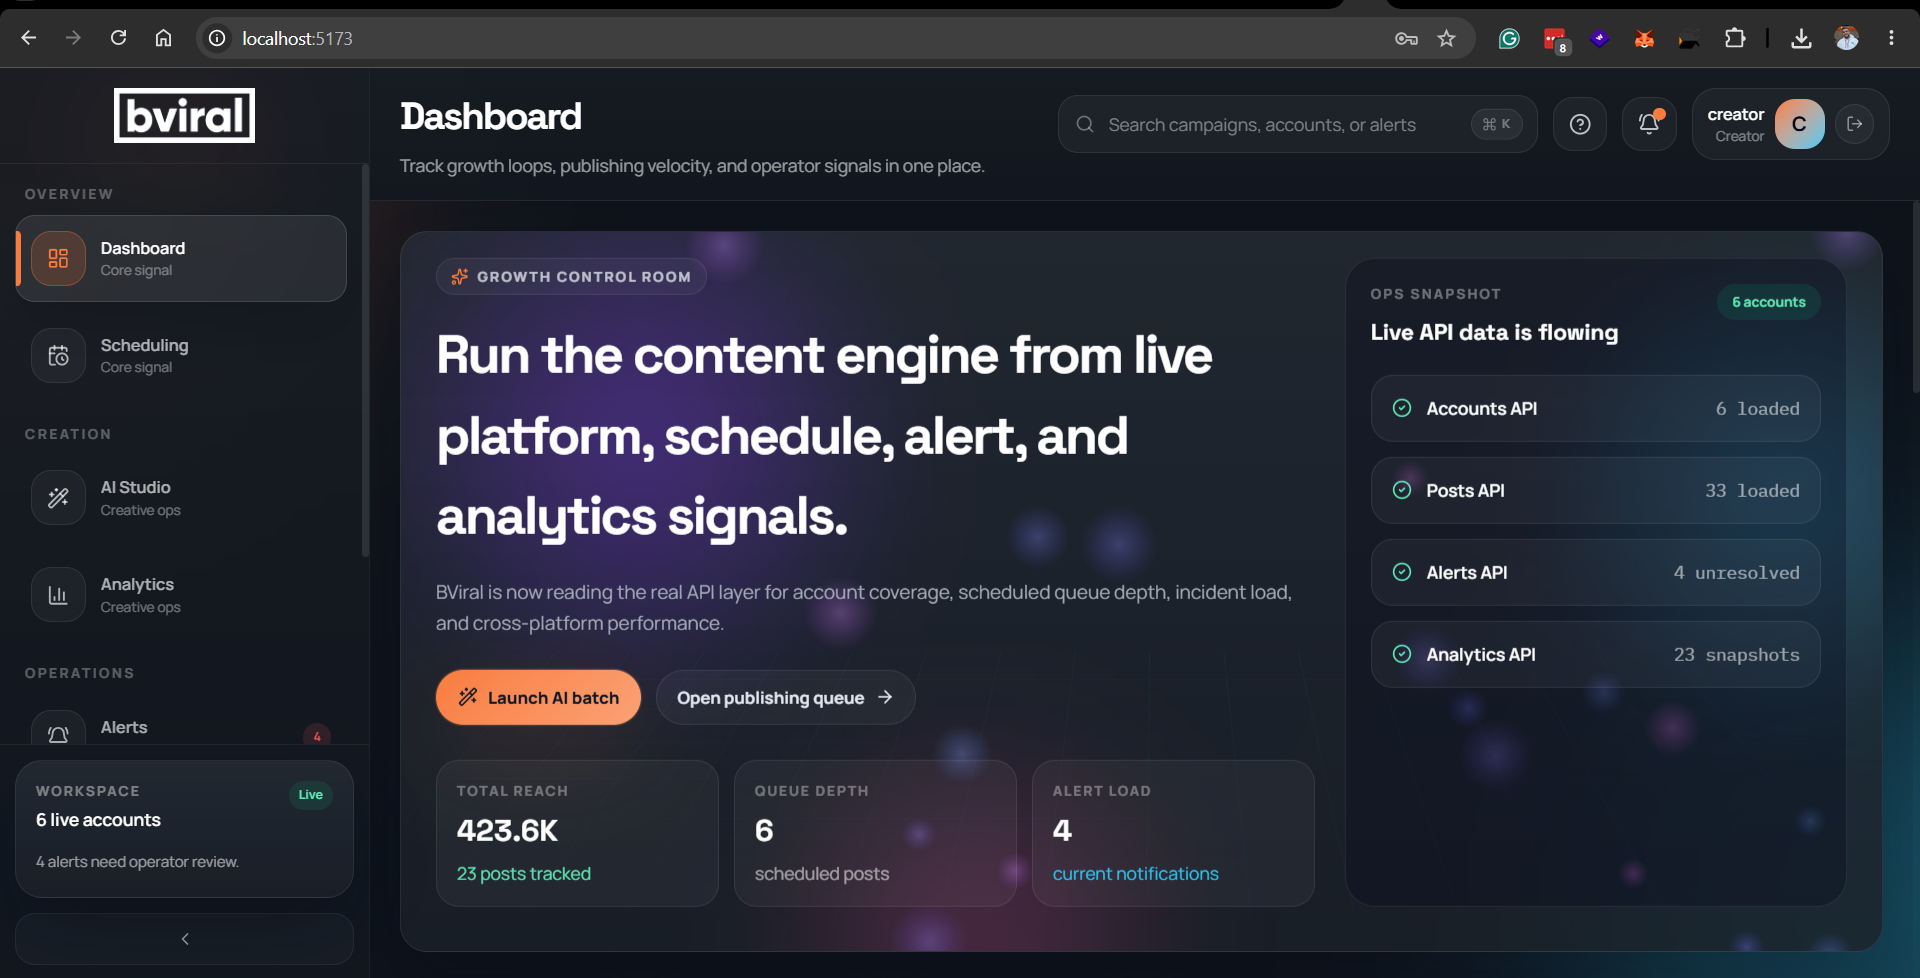
\includegraphics[width=\textwidth]{screens/Home.png}
    \caption{Interface: Dashboard overview}
    \label{fig:ui-dashboard}
\end{figure}

\subsection{Video Scheduling}

The scheduling page presents a visual calendar interface where creators can view, create, and manage scheduled posts. A side panel allows creating new posts by selecting a video, target platform, connected account, and schedule time. Posts are color-coded by status: blue for scheduled, green for posted, and red for failed.

\begin{figure}[H]
    \centering
    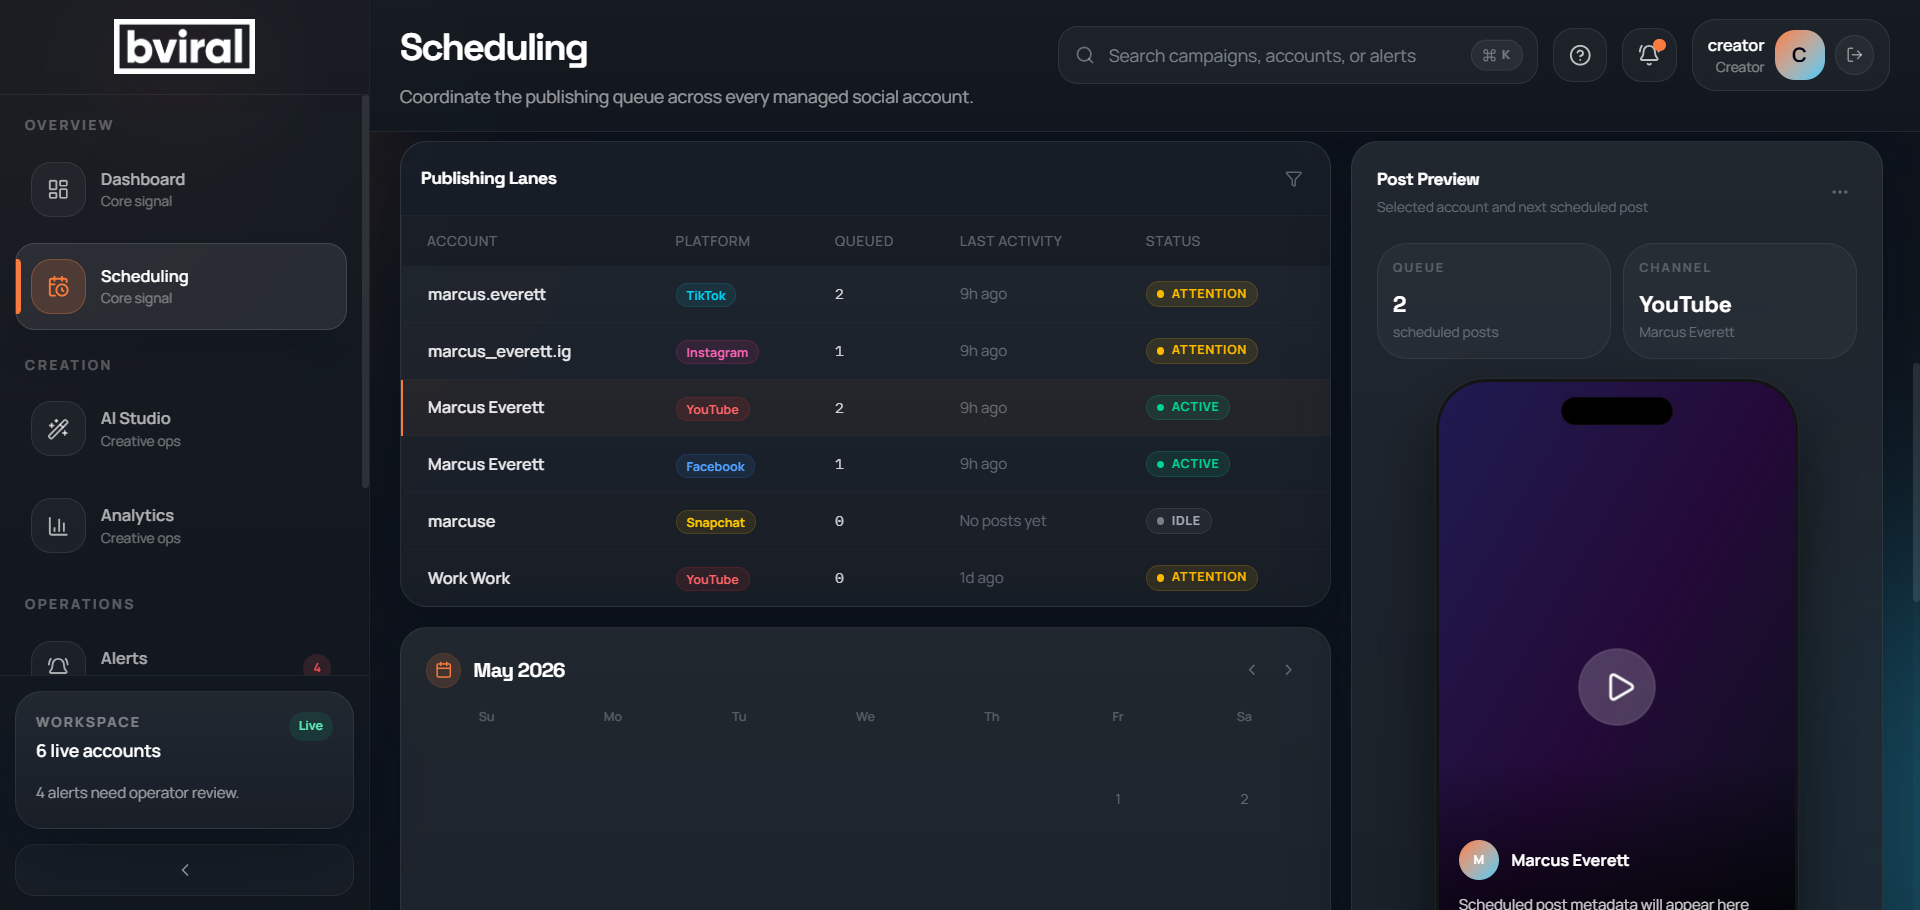
\includegraphics[width=\textwidth]{screens/scheduling.png}
    \caption{Interface: Video scheduling calendar}
    \label{fig:ui-scheduling}
\end{figure}

\subsection{Account Management}

The accounts page displays all connected social media accounts organized by platform. Each account card shows the platform icon, account name, and connection status. ``Connect'' buttons initiate the OAuth flow for each supported platform (YouTube, TikTok, Meta).

\begin{figure}[H]
    \centering
    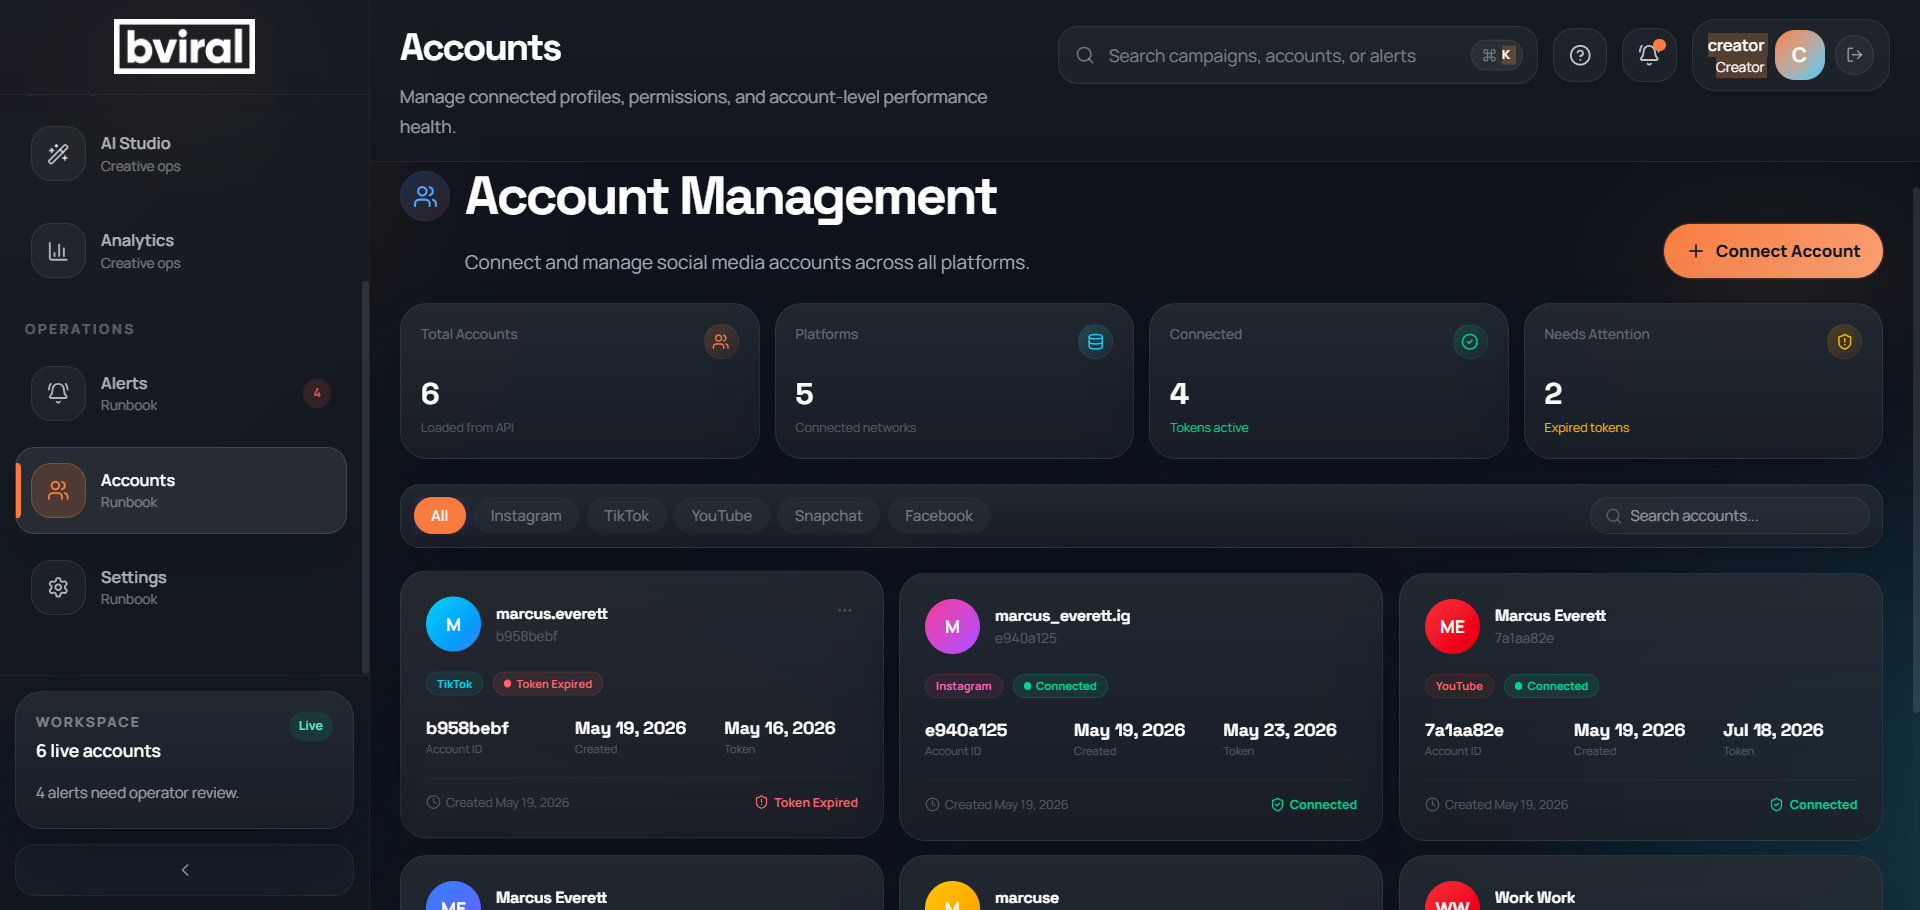
\includegraphics[width=\textwidth]{screens/accounts.png}
    \caption{Interface: Account management}
    \label{fig:ui-accounts}
\end{figure}

\subsection{Analytics Dashboard}

The analytics page provides comprehensive performance monitoring with interactive charts and filters. Users can view aggregated metrics (views, likes, comments, shares, revenue), filter by platform and time period, and visualize engagement trends through line charts, bar charts, and pie charts.

\begin{figure}[H]
    \centering
    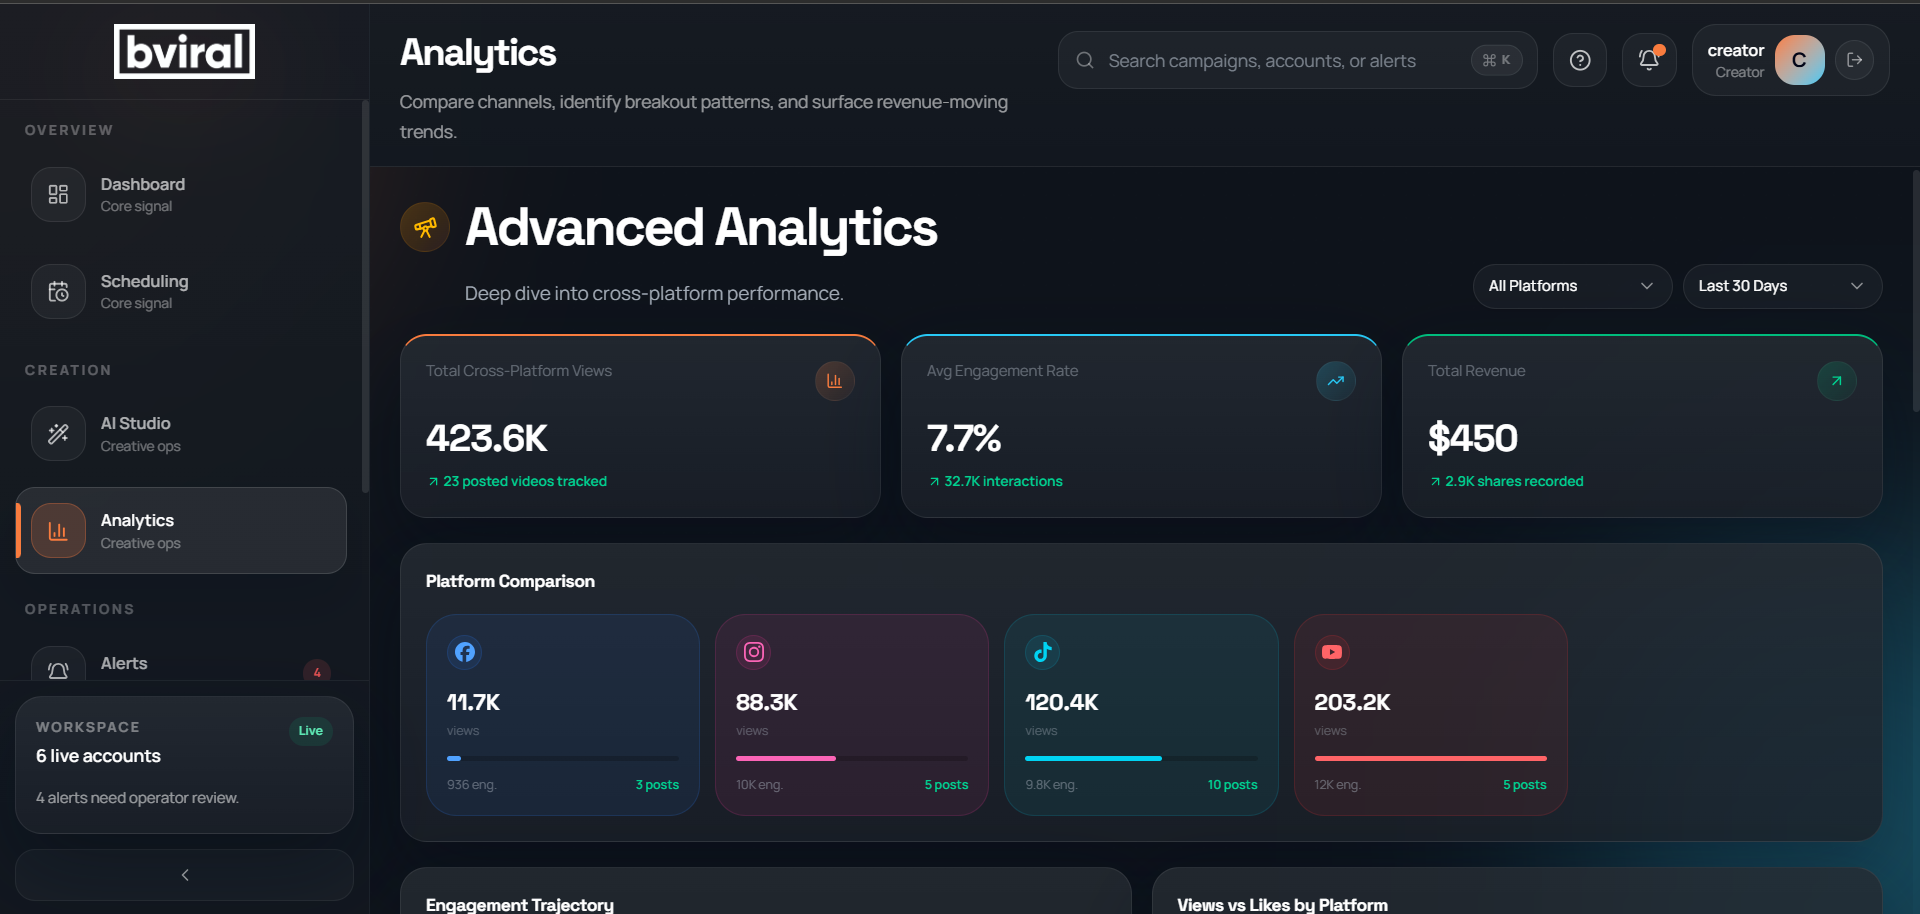
\includegraphics[width=\textwidth]{screens/analytics.png}
    \caption{Interface: Analytics dashboard}
    \label{fig:ui-analytics}
\end{figure}

\subsection{AI Video Studio}

The AI Video Studio provides access to the video enhancement pipeline and the integrated BVIRAL Video Editor. Users can upload videos, configure enhancement parameters (mode, filters, resolution), and preview results with quality metrics.

\begin{figure}[H]
    \centering
    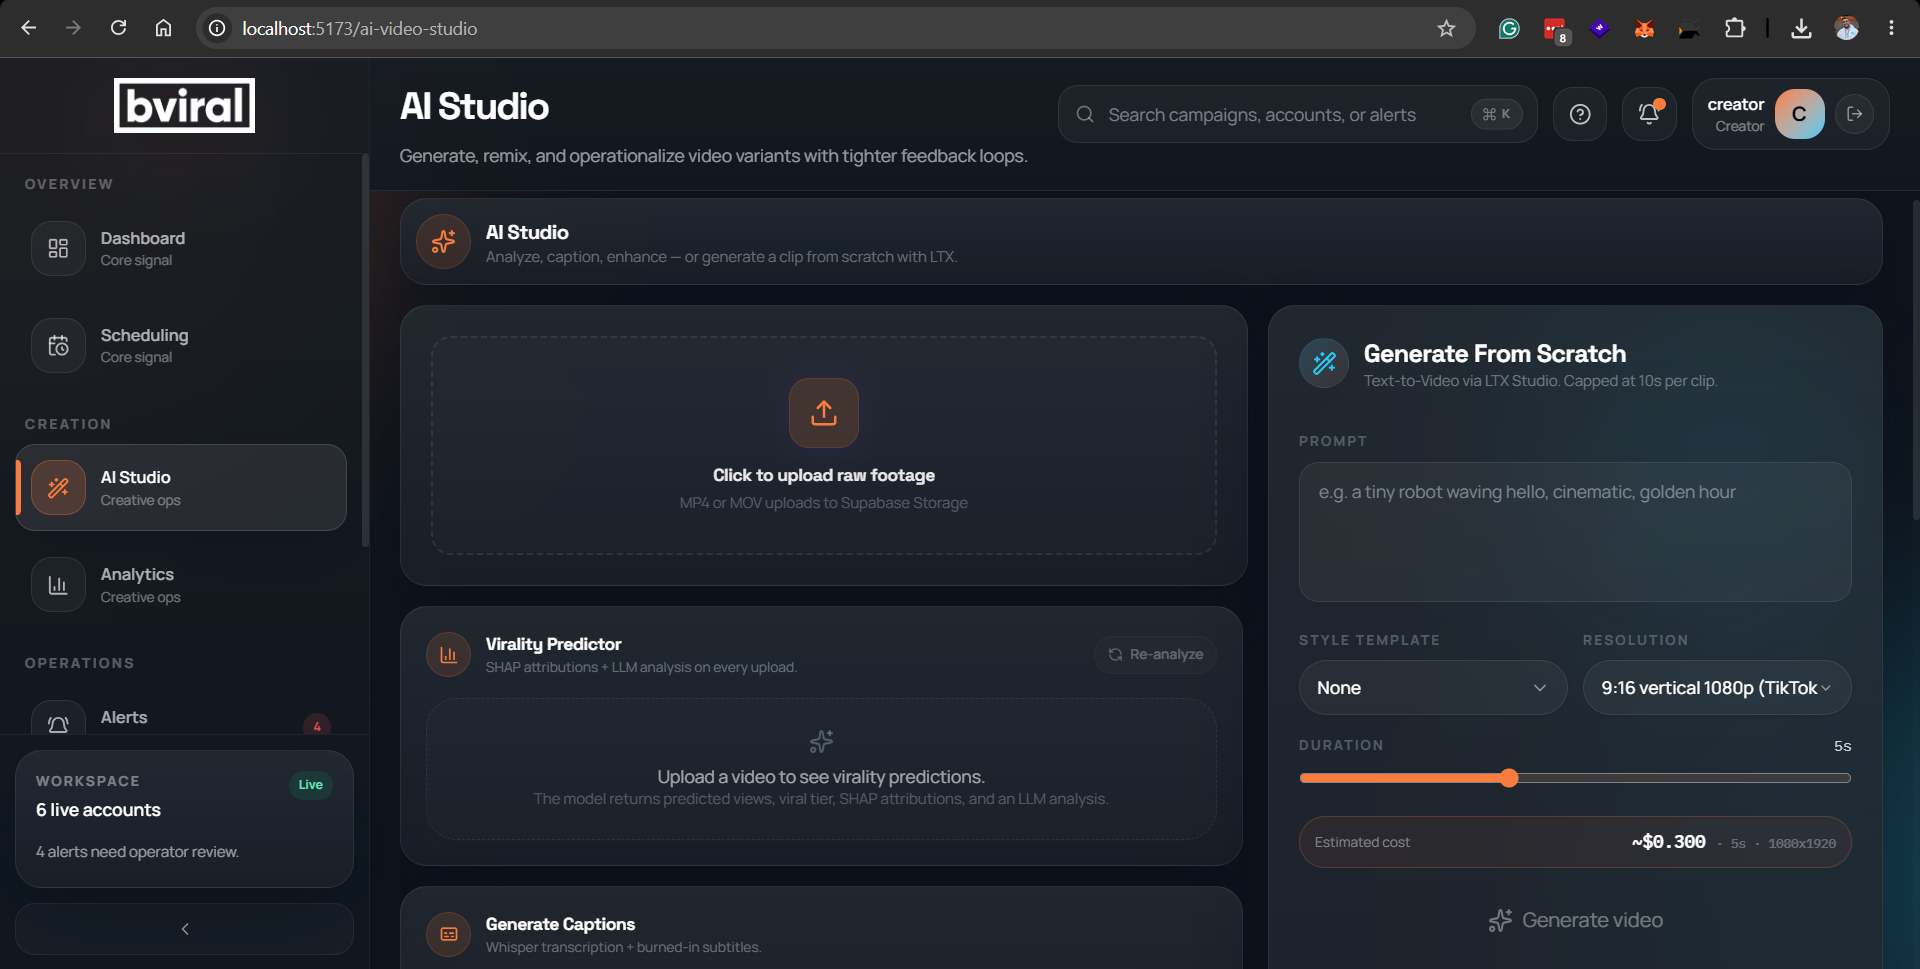
\includegraphics[width=\textwidth]{screens/aistudio.png}
    \caption{Interface: AI Video Studio}
    \label{fig:ui-ai-studio}
\end{figure}

\subsection{Alert Management}

The alerts page displays system notifications in a filterable table. Each alert shows its type (error, copyright, success), associated platform, message, and resolution status. Users can mark alerts as resolved or filter by type and status.

\begin{figure}[H]
    \centering
    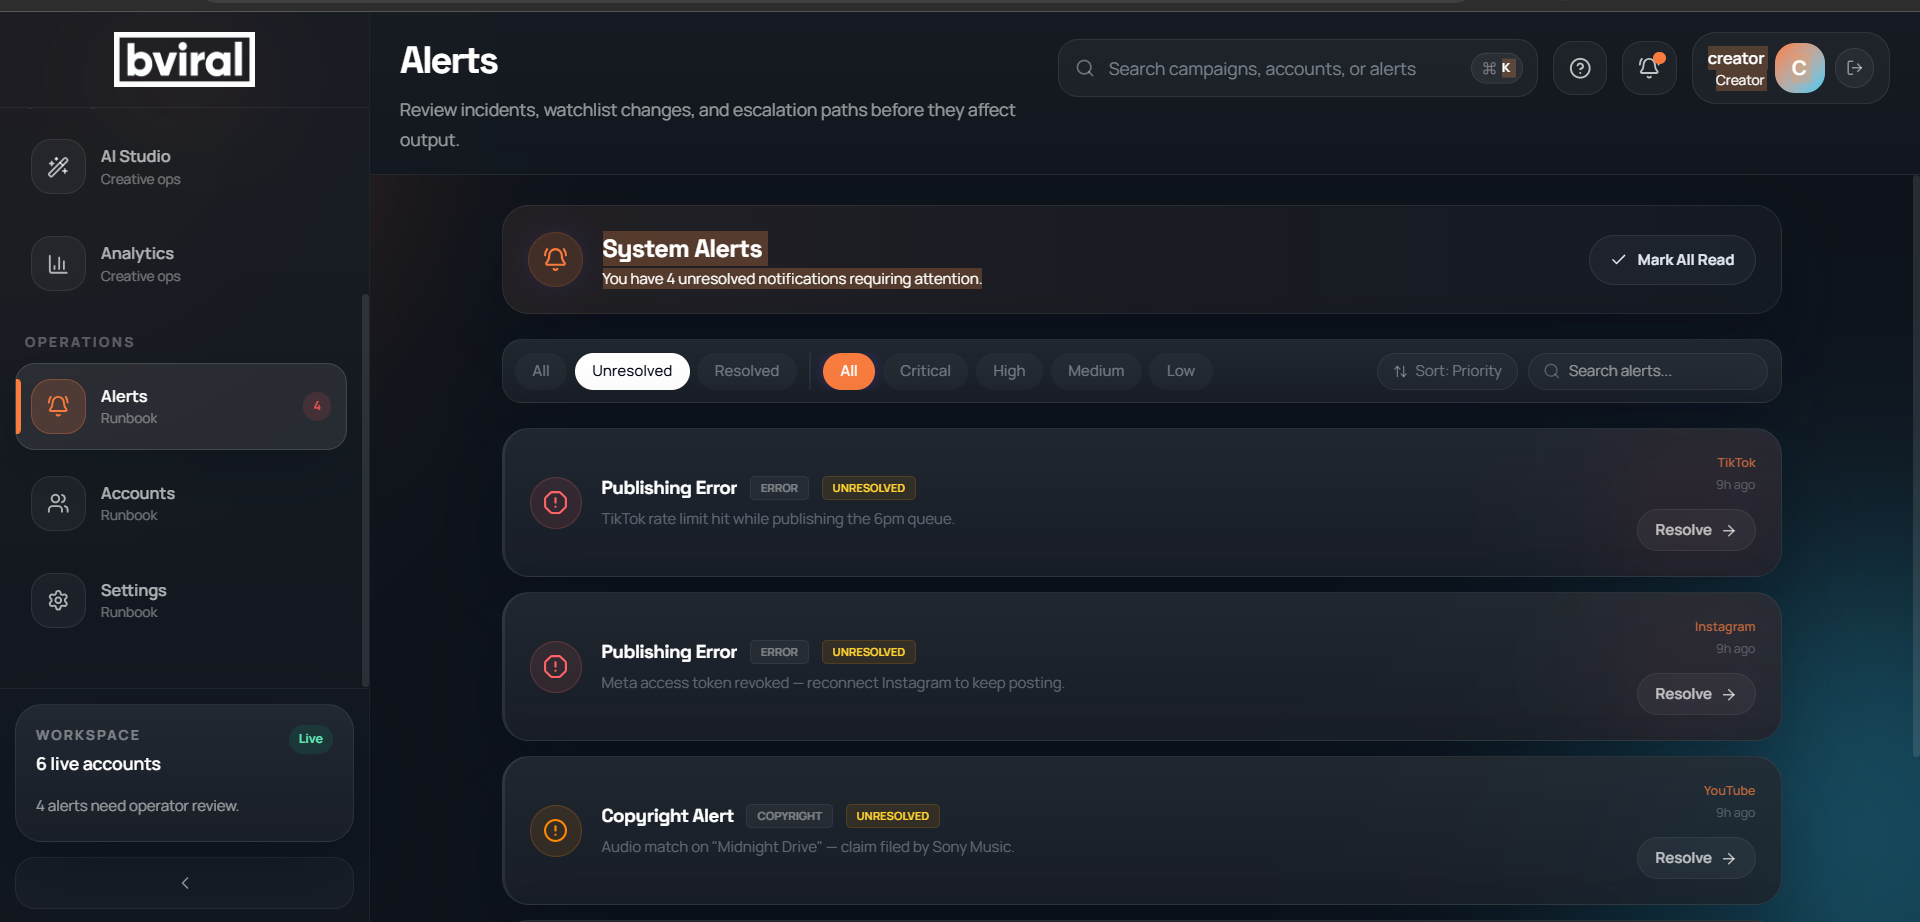
\includegraphics[width=\textwidth]{screens/alerts.png}
    \caption{Interface: Alert management}
    \label{fig:ui-alerts}
\end{figure}

\subsection{Settings}

The settings page allows users to configure their profile, notification preferences, API keys, and system options.

\begin{figure}[H]
    \centering
    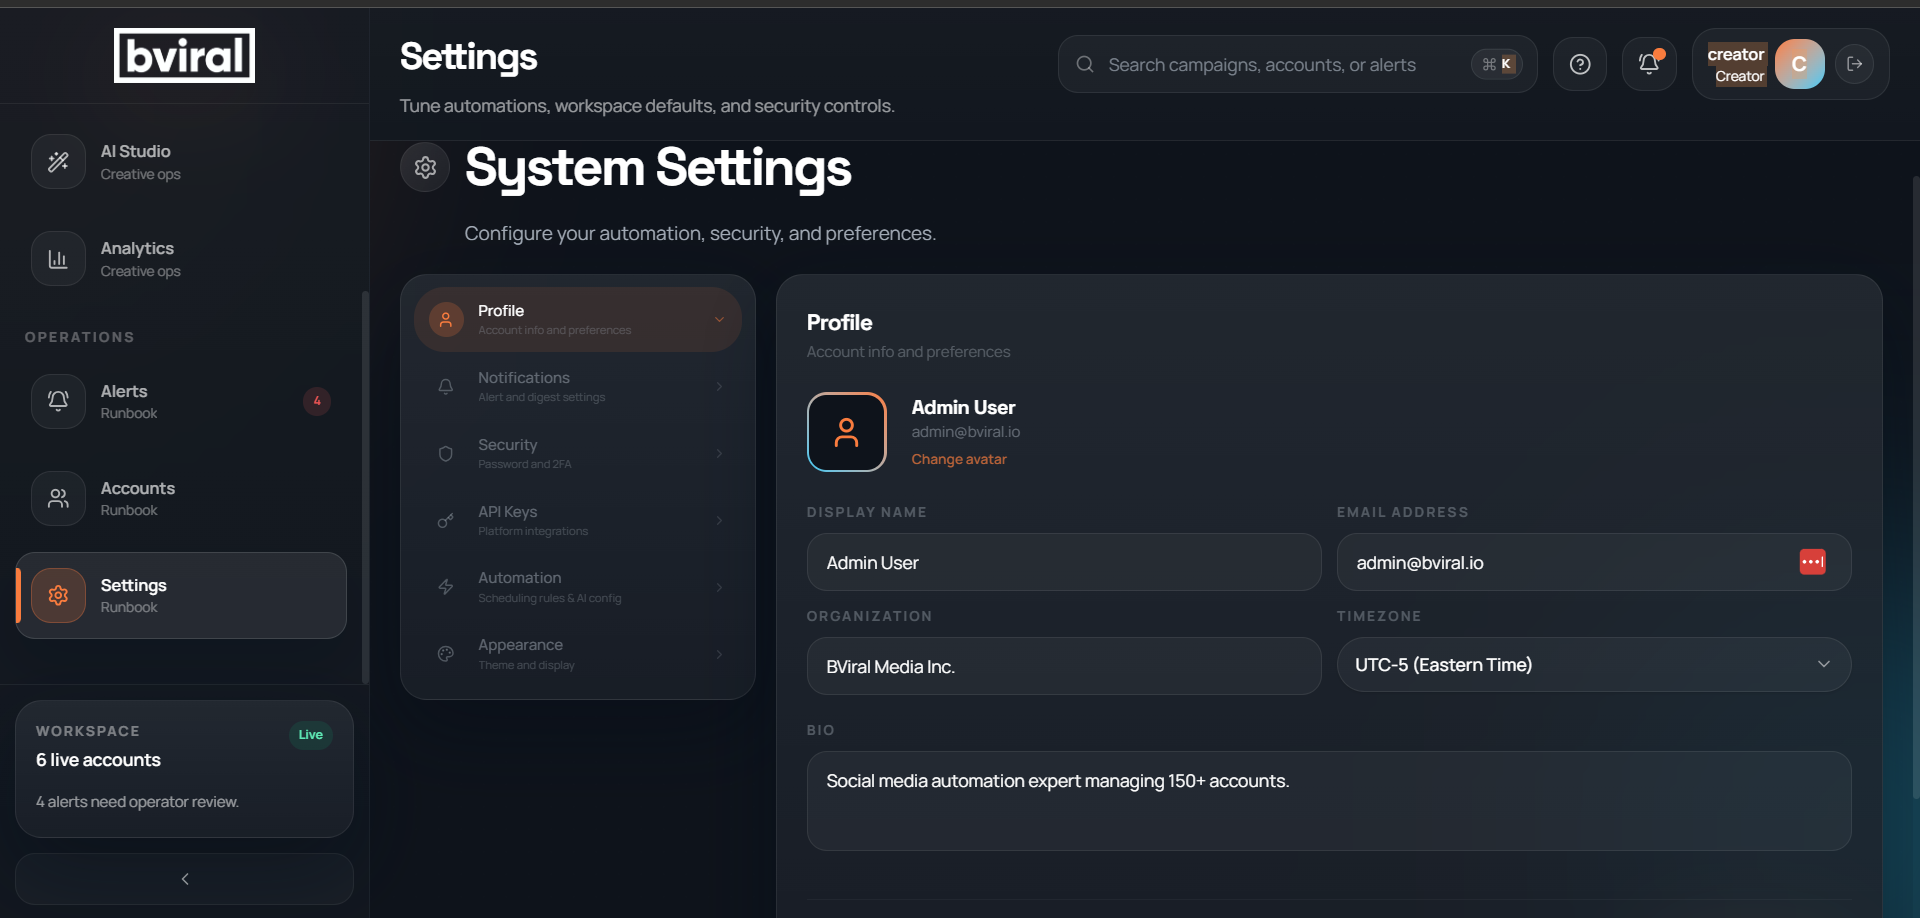
\includegraphics[width=\textwidth]{screens/settings.png}
    \caption{Interface: System settings}
    \label{fig:ui-settings}
\end{figure}

\subsection{Admin Interfaces}

In addition to the creator-facing screens, the dashboard exposes a dedicated admin section accessible only to users with the \texttt{admin} role. Each admin route is guarded both client-side (by the \texttt{AdminOnly} React component) and server-side (by the Fastify \texttt{requireRole("admin")} hook), so a malicious request that bypasses the UI is still rejected at the API layer.

\begin{itemize}
    \item \textbf{Creators:} the administrator can invite, edit, suspend, or remove content creators. A suspended creator can no longer authenticate (the API enforces \texttt{403 Suspended} on every authenticated route except those with the admin role).
    \item \textbf{All Posts:} cross-tenant table of every scheduled or published post in the system, with bulk soft-delete actions.
    \item \textbf{All Videos:} every uploaded video with its owner, derived posts, and processing status.
    \item \textbf{Global Analytics:} aggregated KPIs across all creators with filters, time ranges, and a CSV export.
    \item \textbf{Trash:} posts removed by an admin enter a soft-delete state (column \texttt{deletedAt} populated). The Trash page lets the administrator restore them within the retention window or purge them permanently.
    \item \textbf{Audit Log:} immutable read-only view of the \texttt{admin\_audit\_log} table. Each row exposes the admin, the action, the affected entity, and the JSON payload.
    \item \textbf{System Health:} queue depth and failed-job inspection for the four BullMQ queues, with a one-click retry endpoint.
\end{itemize}

% ══════════════════════════════════════════════════════════════
\section{Security Architecture}
% ══════════════════════════════════════════════════════════════

Security is treated as a cross-cutting concern of the platform rather than a single feature. The design relies on three layered defences: a verified JWT-based authentication, database-level Row-Level Security, and at-rest encryption of every OAuth credential.

\subsection{Supabase JWT Authentication and Role Resolution}

The dashboard performs sign-in against Supabase Auth and stores the returned JWT in the browser session. Each request to the API includes this token in the \texttt{Authorization: Bearer ...} header. The \texttt{50-auth} plugin verifies the token by calling \texttt{<SUPABASE\_URL>/auth/v1/user}, then resolves an internal role using the following priority:

\begin{enumerate}
    \item Explicit claim in the token's \texttt{app\_metadata} (\texttt{app\_role}, \texttt{role}, \texttt{user\_role}, or \texttt{team\_role}) equal to \texttt{admin}.
    \item Otherwise, the \texttt{role} column of the local \texttt{users} table.
    \item Otherwise, the default role \texttt{content\_creator}.
\end{enumerate}

If the resolved user carries a non-null \texttt{suspendedAt} and is not an admin, the request is rejected with \texttt{403 Forbidden}. For local development only, a \texttt{ADMIN\_TOKEN} environment variable enables an automatic admin user attachment to streamline the developer experience; this shortcut is explicitly disabled when \texttt{NODE\_ENV=production}.

\subsection{Row-Level Security (RLS)}

Every business table (\texttt{users}, \texttt{accounts}, \texttt{videos}, \texttt{posts}, \texttt{analytics}, \texttt{alerts}, \texttt{admin\_audit\_log}) has RLS enabled at the PostgreSQL level, with Drizzle-generated \texttt{pgPolicy} declarations. Two families of policies coexist:

\begin{itemize}
    \item \texttt{<table>\_select\_own / insert\_own / update\_own / delete\_own}: a user can only see or modify rows they own (resolved via \texttt{auth.uid()}).
    \item \texttt{admins\_full\_access\_<table>}: a JWT with the \texttt{app\_role = admin} claim is granted full access.
\end{itemize}

This provides defence-in-depth: even if the API layer were compromised or a query forgot a \texttt{WHERE userId = ...} filter, PostgreSQL itself would still refuse to return rows that do not belong to the authenticated user.

\subsection{OAuth Token Encryption at Rest (AES-256-GCM)}

OAuth access and refresh tokens stored in the \texttt{accounts} table are encrypted before persistence using AES-256-GCM, implemented in \texttt{lib/token-encryption.ts}. The storage format is versioned:

\begin{center}
\texttt{enc:v1:<base64url(iv)>:<base64url(authTag)>:<base64url(ciphertext)>}
\end{center}

The encryption key is loaded from the \texttt{TOKEN\_ENCRYPTION\_KEY} environment variable (base64, hex, or a passphrase derived via SHA-256). In production, a missing key causes the API to fail fast at startup. In development, the code falls back to a stable derived key and emits a one-time warning. Legacy plaintext tokens are detected via the absence of the \texttt{enc:v1:} prefix and silently re-encrypted on the next write.

\subsection{TikTok PKCE and Multi-Provider OAuth}

The platform integrates with three OAuth providers (YouTube/Google, TikTok, and Meta for Facebook \& Instagram). TikTok additionally requires PKCE (Proof Key for Code Exchange) and refuses \texttt{localhost} redirect URIs. The implementation keeps the per-attempt PKCE verifier in API memory, and in local development the dashboard is tunneled through \texttt{ngrok} so TikTok accepts the HTTPS redirect URL. Each provider has its own environment configuration; missing credentials return a clean \texttt{503 Service Unavailable} instead of crashing the server.

\subsection{Log Redaction and Sensitive Data Handling}

In production, the Pino logger is configured with a redact list covering \texttt{authorization}, \texttt{cookie}, \texttt{x-admin-token}, \texttt{body.password}, \texttt{*.password}, \texttt{*.secret}, and \texttt{*.token}. This prevents accidental leakage of bearer tokens or user credentials through log aggregation pipelines.

\subsection{Admin Audit Trail}

Every administrative write goes through a single helper, \texttt{writeAudit()}, which inserts a row into the \texttt{admin\_audit\_log} table with the admin id, the action name (e.g.\ \texttt{system.retry\_job}, \texttt{creator.suspend}, \texttt{post.soft\_delete}), the target type, the target id, and a JSON payload describing the operation. The Audit Log admin page is a thin read-only view over this table; the table is indexed on \texttt{(adminId, createdAt)} and \texttt{(targetType, targetId)} for fast forensic lookups.

% ══════════════════════════════════════════════════════════════
\section{Asynchronous Processing and Job Queues}
% ══════════════════════════════════════════════════════════════

Long-running and time-deferred work is delegated to BullMQ workers backed by Redis, keeping the HTTP request path responsive and allowing horizontal scaling of the background fleet.

\subsection{Queue Topology}

Four distinct queues are declared:

\begin{itemize}
    \item \textbf{\texttt{post-publishing}} --- delayed jobs created at the scheduled publication time of each post. Consumed by \texttt{workers/posts.worker.ts}.
    \item \textbf{\texttt{video-processing}} --- video enhancement, super-resolution, and re-encoding jobs. Consumed by \texttt{workers/videos.worker.ts}.
    \item \textbf{\texttt{analytics-refresh}} --- a repeatable cron-style job (\texttt{analyticsRefreshCronPattern}) that pulls fresh metrics from each platform every six hours. Consumed by \texttt{workers/analytics.worker.ts}.
    \item \textbf{\texttt{ai-processing}} --- caption generation, virality prediction, and LTX text-to-video jobs. Consumed by \texttt{workers/ai.worker.ts}.
\end{itemize}

\subsection{Self-Healing on Boot}

When the publishing worker starts, it scans the database for posts whose status is still \texttt{scheduled} and re-enqueues them, including posts that became overdue while the worker was off. This makes the system tolerant to worker restarts, deployments, and short outages without manual intervention.

\subsection{Operational Visibility and Retry}

The \texttt{queuesAdmin} decorator exposed by the queues plugin provides three operations consumed by the System Health admin page:

\begin{itemize}
    \item \texttt{getStats()} --- counts of waiting, active, completed, failed, delayed, and paused jobs per queue.
    \item \texttt{getFailedJobs(queueName, limit)} --- inspection of the most recent failed jobs (name, failure reason, attempts, timestamps).
    \item \texttt{retryJob(queueName, jobId)} --- one-click re-enqueue of a specific failed job, with a corresponding audit log entry.
\end{itemize}

% ══════════════════════════════════════════════════════════════
\section{API Specification and Type-Safe Code Generation}
% ══════════════════════════════════════════════════════════════

A recurring source of bugs in client--server applications is drift between the contract documented by the backend and the assumptions made by the frontend. To eliminate this drift, the BViral codebase treats the OpenAPI 3.1 specification (\texttt{lib/api-spec/openapi.yaml}) as the single source of truth. From this file, two libraries are auto-generated:

\begin{itemize}
    \item \texttt{lib/api-zod} --- runtime Zod validation schemas, consumed by the Fastify route handlers and the workers for inbound payload validation.
    \item \texttt{lib/api-client-react} --- TanStack Query hooks (\texttt{useListPosts}, \texttt{useCreatePost}, \texttt{useListAccounts}, etc.) with full TypeScript types, consumed directly by the dashboard.
\end{itemize}

Any change to the OpenAPI specification regenerates both libraries; the TypeScript compiler then surfaces every call site that needs to be updated. This guarantees compile-time and runtime alignment between the API and its only first-party client.

% ══════════════════════════════════════════════════════════════
\section{Multi-Platform Publishing Abstraction}
% ══════════════════════════════════════════════════════════════

The diversity of social-media APIs (YouTube Data API, TikTok Open API, Meta Graph API) is hidden behind a single \texttt{platform-publisher.service}. Each provider has its own service (\texttt{youtube.service}, \texttt{tiktok.service}, \texttt{meta.service}) implementing a uniform \texttt{publish(post, account, video)} interface. The publishing worker dispatches a job to the correct provider based on the \texttt{platform} column of the post. New providers (e.g.\ Snapchat) can be added with no change to the worker or to the API contract --- the database enum already includes the platform value.

% ══════════════════════════════════════════════════════════════
\section{AI Component Design}
% ══════════════════════════════════════════════════════════════

The artificial intelligence ecosystem within BViral Control Center is structured around three independent but complementary pillars: the Pre-Posting Predictive Agent, the Auto-Captioning Engine, and the Video Quality Enhancement Engine.

\begin{figure}[H]
    \centering
    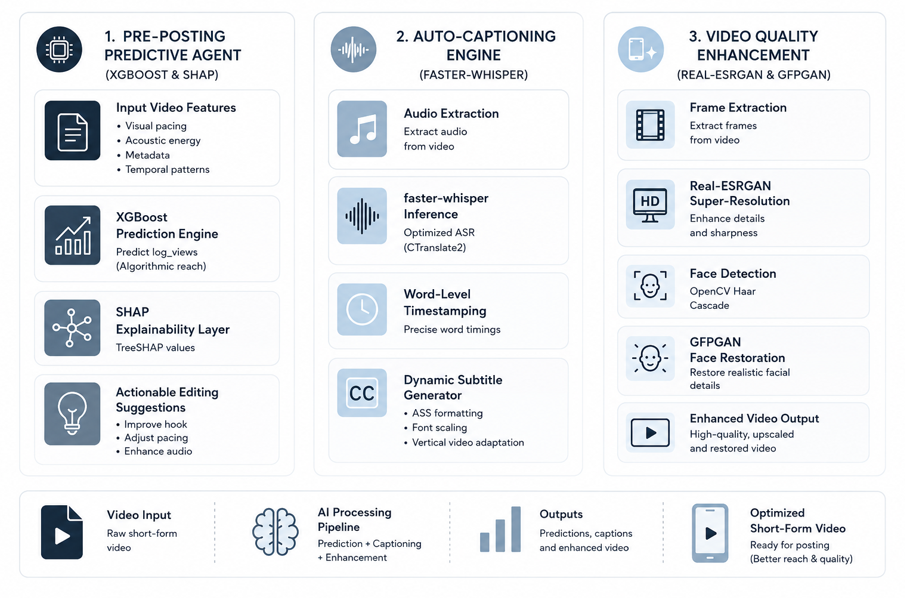
\includegraphics[width=0.8\textwidth]{images/aidesign.png}
    \caption{AI component design of BViral Control Center}
    \label{fig:ai_design}
\end{figure}

\subsection{Algorithm Selection and Justification}

Each pillar utilizes specific algorithms chosen for their performance, hardware efficiency, and suitability for the task:

\begin{itemize}
    \item \textbf{Pillar 1: Pre-Posting Predictive Agent (XGBoost \& SHAP):} 
    To predict a video's algorithmic reach (\texttt{log\_views}), we selected \textbf{XGBoost (eXtreme Gradient Boosting)}. Unlike Deep Neural Networks which are prone to overfitting on tabular data of this size ($\sim$1,100 rows), XGBoost excels at capturing complex, non-linear interactions between multimodal features (e.g., visual pacing vs. acoustic energy). Crucially, XGBoost integrates flawlessly with \textbf{TreeSHAP} (SHapley Additive exPlanations), allowing the system to reverse-engineer the prediction and provide explainable, actionable editing advice to the creator.
    
    \item \textbf{Pillar 2: Auto-Captioning Engine (\texttt{faster-whisper}):}
    Standard OpenAI Whisper models are highly accurate but computationally heavy. We justified the use of \texttt{faster-whisper},a reimplementation that drastically reduces VRAM usage while running up to 4 times faster. It extracts precise word-level timestamps, which are then passed to a custom font-scaling algorithm to dynamically generate \texttt{.ass} subtitle scripts formatted specifically for short-form vertical screens.
    
    \item \textbf{Pillar 3: Video Quality Enhancement (Real-ESRGAN \& GFPGAN):}
    For super-resolution, we selected \textbf{Real-ESRGAN}, a Generative Adversarial Network optimized for restoring real-world degraded videos by hallucinating missing high-frequency details. Because standard GANs often distort human faces, we integrated \textbf{GFPGAN} as a secondary pass specifically triggered by OpenCV Haar Cascade face detection. GFPGAN leverages generative facial priors to reconstruct realistic eyes, teeth, and skin textures.
\end{itemize}



% ══════════════════════════════════════════════════════════════
\section*{Conclusion}
% ══════════════════════════════════════════════════════════════

In this chapter, we presented the technical architecture of BViral Control Center, justified our technology choices, and showcased the implemented interfaces. The monorepo workspace architecture provides a clean separation between the React dashboard and the Fastify API server. Furthermore, the integration of a highly complex, three-pillar AI ecosystem—featuring an XGBoost Predictive Agent, a Whisper-driven Auto-Captioning engine, and a Real-ESRGAN/GFPGAN enhancement pipeline distinguishes our solution from standard social media management tools by offering creator-focused algorithmic diagnostics and production-grade video processing.

\phantomsection
\addcontentsline{toc}{section}{Conclusion}



\chapter[AI Component: Experiments and Evaluation]{AI Component: Experiments and~Evaluation}

\section*{Introduction}
\phantomsection
\addcontentsline{toc}{section}{Introduction}
This chapter constitutes the scientific core of the AI component. It presents the full experimental methodology, beginning with Exploratory Data Analysis (EDA) of the collected dataset, followed by the validation of the multimodal feature extraction pipeline. It then reports model training and evaluation results using regression metrics, learning curves, and SHAP explainability, in order to rigorously demonstrate the reliability of the Pre‑Posting Predictive Agent.

\section{Dataset Description and Data Collection}
To train the Pre-Posting Predictive Agent, a custom multimodal dataset was constructed, since no public dataset provides both raw short-form videos and their algorithmic reach metrics.

\begin{itemize}
    \item \textbf{Sources:} TikTok, YouTube Shorts, and Instagram Reels.
    \item \textbf{Collection Method:} Automated scraping using \texttt{yt-dlp} and platform-specific scripts to download both \texttt{.mp4} files and metadata.
    \item \textbf{Size and Format:} $\sim$1,100 raw videos stored as \texttt{.mp4}, accompanied by a unified metadata table (\texttt{all\_metadata.csv}) containing fields such as \texttt{video\_id}, \texttt{title}, \texttt{platform}, \texttt{duration\_seconds}, \texttt{views}, \texttt{upload\_date}, and \texttt{local\_video\_path}.
    \item \textbf{Multimodal Outputs:} Each video is processed into separate feature artifacts: 
    \begin{itemize}
        \item \textbf{Visual Embeddings:} CLIP vectors for hook and full video (\texttt{.npy} files).
        \item \textbf{Audio Features:} Librosa acoustic descriptors (RMS, tempo, MFCCs, silence ratio) saved as JSON.
        \item \textbf{Transcripts:} Whisper ASR output (hook + full transcript) stored as JSON.
        \item \textbf{Textual Embeddings:} SentenceTransformer vectors for combined title + transcript.
        \item \textbf{LLM Annotations:} Llama/Groq semantic labels (tone, hook type, scores), structured as JSON.
    \end{itemize}
    \item \textbf{Data Cleaning:} Duplicate \texttt{video\_id}s were removed prior to splitting to prevent leakage. Videos with corrupted audio or missing files were discarded, and silent videos were kept but labeled with empty transcripts.
\end{itemize}

% ══════════════════════════════════════════════════════════════
\section{Exploratory Data Analysis (EDA)}
% ══════════════════════════════════════════════════════════════
Before training, we conducted a rigorous EDA on the combined dataset of $\sim$1,100 short-form videos to understand the underlying statistical distributions and correlations.

\subsection{Target Variable Transformation}
Social media views naturally follow an exponential power-law distribution. Most videos receive very few views, while a small minority go massively viral. 

\begin{figure}[H]
    \centering
    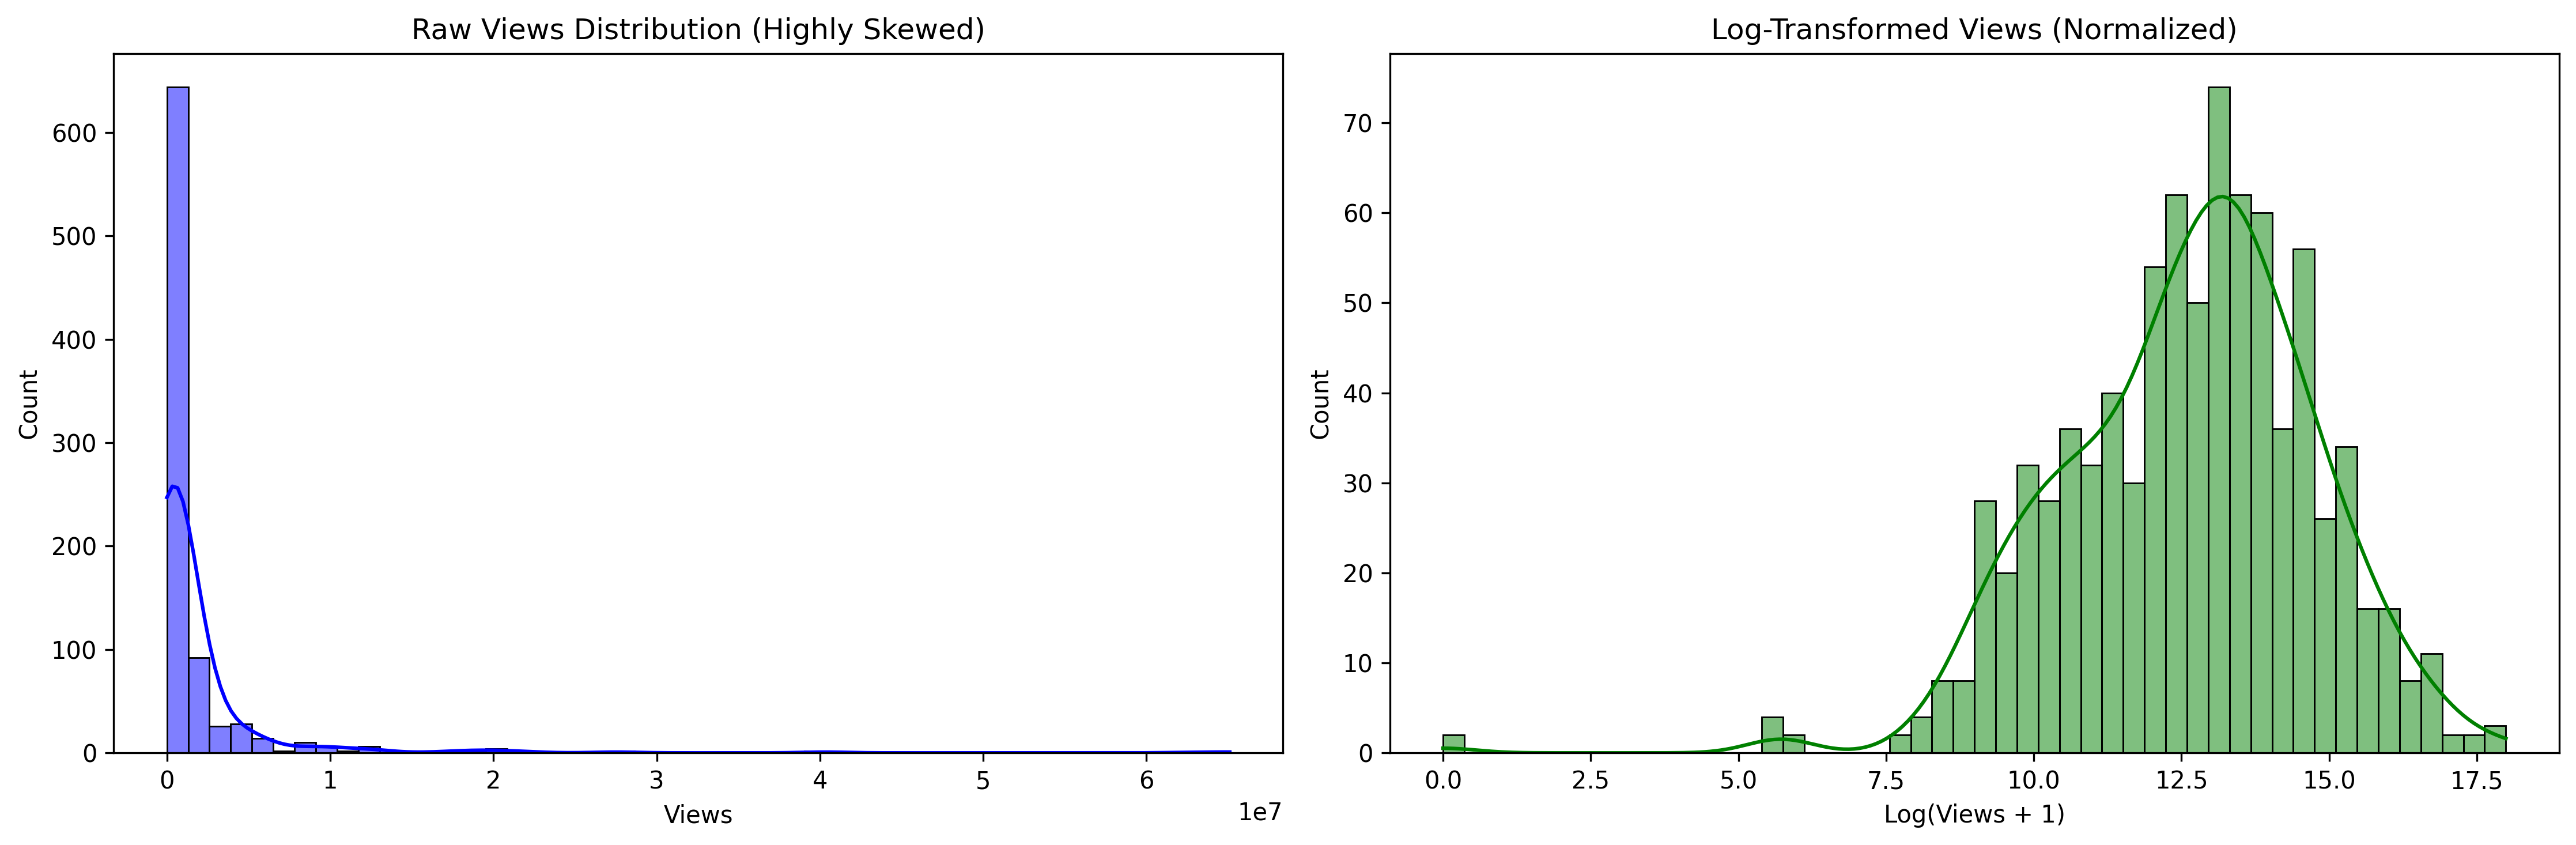
\includegraphics[width=0.9\textwidth]{images/target_distribution.png}
    \caption{Distribution of raw views (left) versus the Log-Transformed target variable (right).}
    \label{fig:eda_distribution}
\end{figure}

As observed in Figure \ref{fig:eda_distribution}, the raw view counts are heavily right-skewed. To prevent the regression model from being disproportionately penalized by these viral outliers, a logarithmic transformation (\texttt{numpy.log1p}) was applied. This successfully transformed the target variable (\texttt{log\_views}) into a Gaussian-like distribution, stabilizing the loss function during training.

\subsection{Feature Correlation Analysis}
To investigate linear relationships, we generated a Pearson Correlation Matrix comparing our extracted features against \texttt{log\_views}.

\begin{figure}[H]
    \centering
    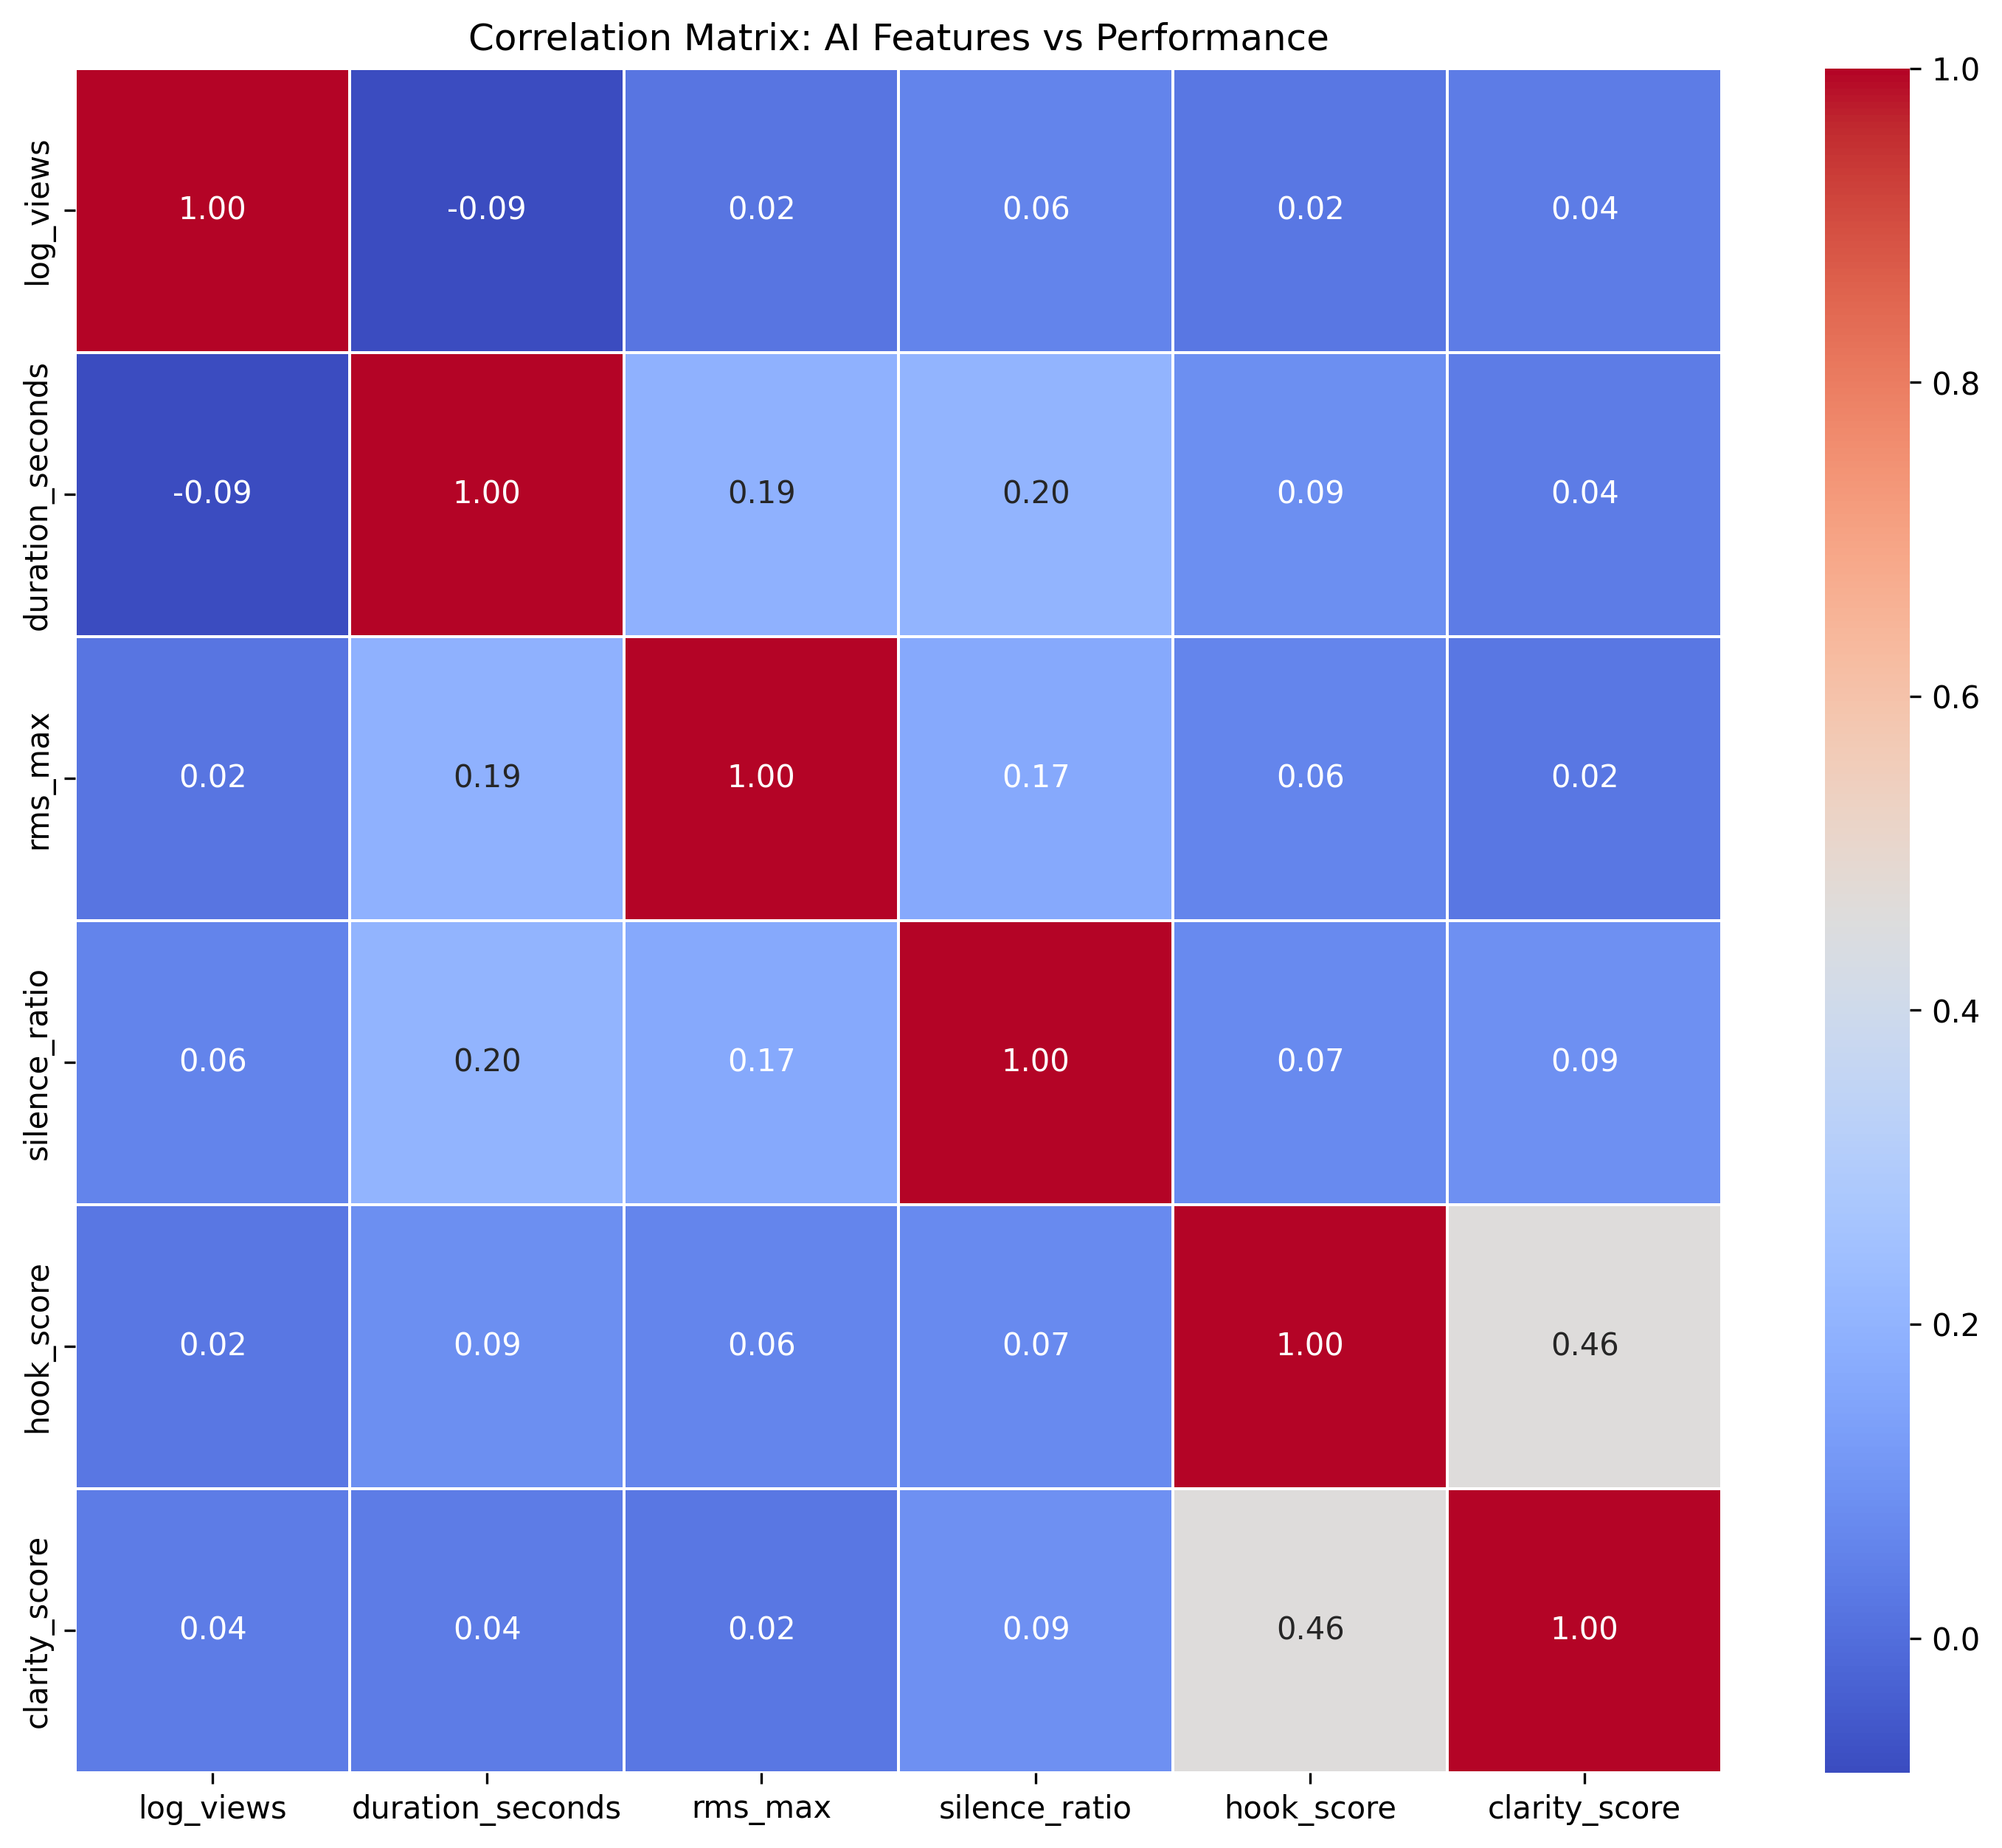
\includegraphics[width=0.4\textwidth]{images/correlation_matrix.png}
    \caption{Pearson Correlation Matrix of AI features vs algorithmic reach (\texttt{log\_views}).}
    \label{fig:eda_correlation}
\end{figure}

Figure \ref{fig:eda_correlation} reveals that no single feature has a strong linear correlation with \texttt{log\_views} (values hovering near zero). This critical finding proves that virality cannot be predicted using simple linear regression. Instead, it justifies our architectural decision to utilize XGBoost, a tree-based ensemble capable of mapping highly complex, non-linear interactions across multiple modalities.

% ══════════════════════════════════════════════════════════════
\section{Feature Extraction \& Dimensionality Reduction}
% ══════════════════════════════════════════════════════════════
The dataset is composed of raw \texttt{.mp4} videos and metadata, which cannot be used directly by machine learning models. Therefore, a dedicated multimodal extraction pipeline was designed to transform each video into structured numerical representations across visual, audio, and semantic modalities. This section details the extraction stages and provides visual evidence to validate the correctness and consistency of the resulting features.
\subsection{Acoustic Extraction (Librosa)}
The first three seconds of a video (the “Hook”) strongly influence viewer retention.\\  To capture these early‑stage acoustic signals, we extracted a short audio window and computed multiple low‑level descriptors using \texttt{librosa}. \\ 
These include RMS energy (loudness), zero‑crossing rate (signal roughness), spectral centroid and roll‑off (brightness), tempo (pacing), silence ratio (dead‑air detection), and MFCCs (timbre). Together, these features quantify pacing, clarity, and auditory intensity factors that are directly linked to a viewer’s decision to continue watching.

\begin{figure}[H]
    \centering
    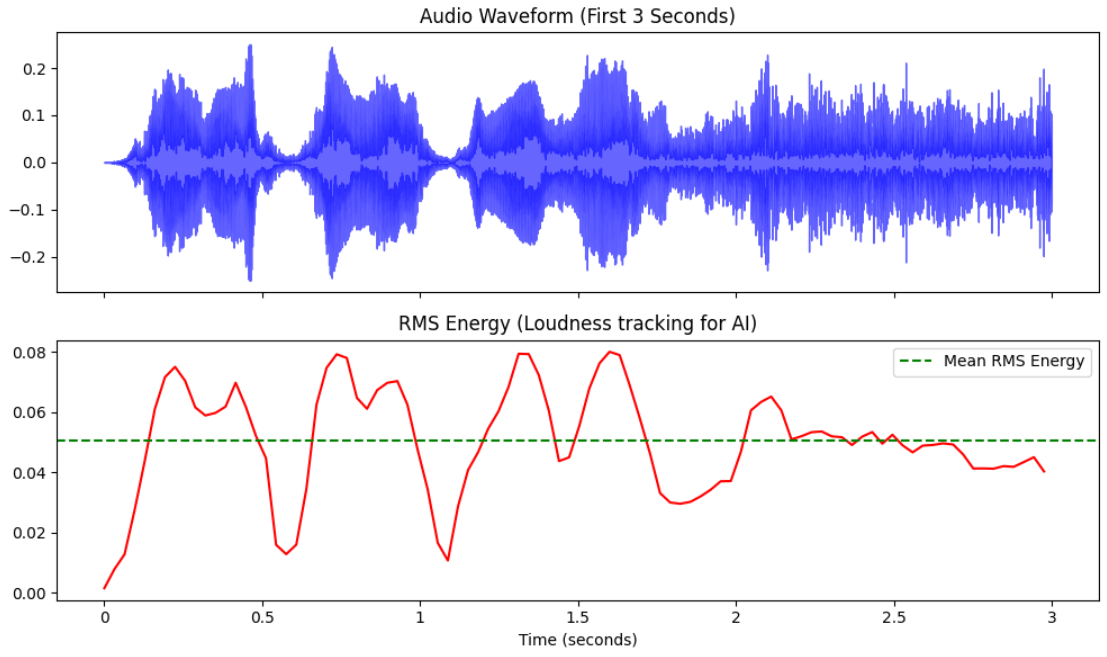
\includegraphics[width=0.8\textwidth]{images/acoustic_features.png}
    \caption{Acoustic feature extraction: Raw audio waveform and RMS Energy.}
    \label{fig:acoustic_features}
\end{figure}

 Figure \ref{fig:acoustic_features}  illustrates how the raw waveform is converted into short‑time energy. RMS energy captures the loudness envelope of the hook, which is critical for detecting silence, weak delivery, or abrupt drop‑offs. We define the \texttt{silence\_ratio} as the proportion of frames whose energy falls below a fixed threshold, enabling the model to quantify “dead air.” This metric is especially important in short‑form content, where low energy in the first seconds strongly predicts early viewer drop‑off.

\begin{figure}[H]
    \centering
    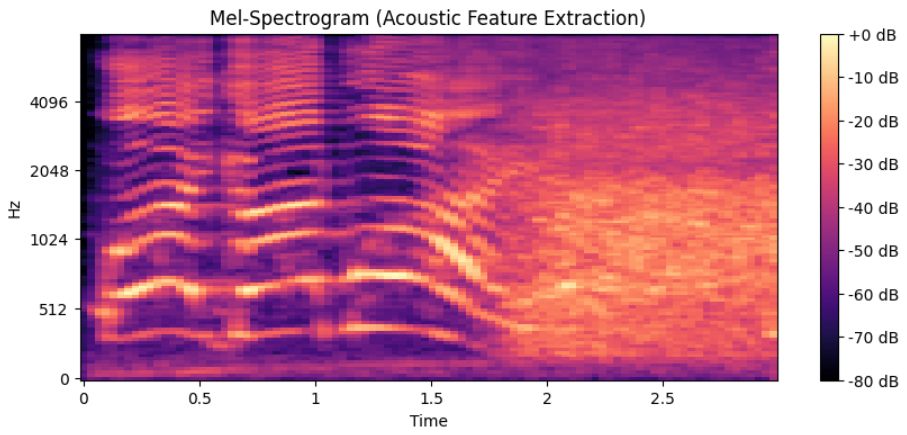
\includegraphics[width=0.7\textwidth]{images/mel_spectrogram.png}
    \caption{Mel-Spectrogram of a 3-second hook, used to extract MFCCs.}
    \label{fig:mel_spectrogram}
\end{figure}

 Figure  \ref{fig:mel_spectrogram} visualizes the Mel‑Spectrogram, which represents how energy is distributed across perceptual frequency bands over time. From this representation, we compute Mel‑Frequency Cepstral Coefficients (MFCCs), a compact descriptor widely used in speech and audio classification. MFCCs capture vocal timbre, clarity, and articulation patterns, helping the model distinguish between engaging speech, background noise, music, or muffled audio—key factors influencing perceived quality and retention.

\subsection{Semantic Profiling (LLM Zero-Shot)}
The LLM generates a structured semantic profile from the Whisper transcript by assigning a dominant tone category (e.g., educational, humorous, inspirational) and extracting high‑level intent signals. These labels convert unstructured language into categorical variables that are later one‑hot encoded. The distribution in the figure indicates which narrative styles dominate the dataset and provides interpretability: the model can be traced to psychological framing choices rather than only low‑level audiovisual patterns.

\begin{figure}[H]
    \centering
    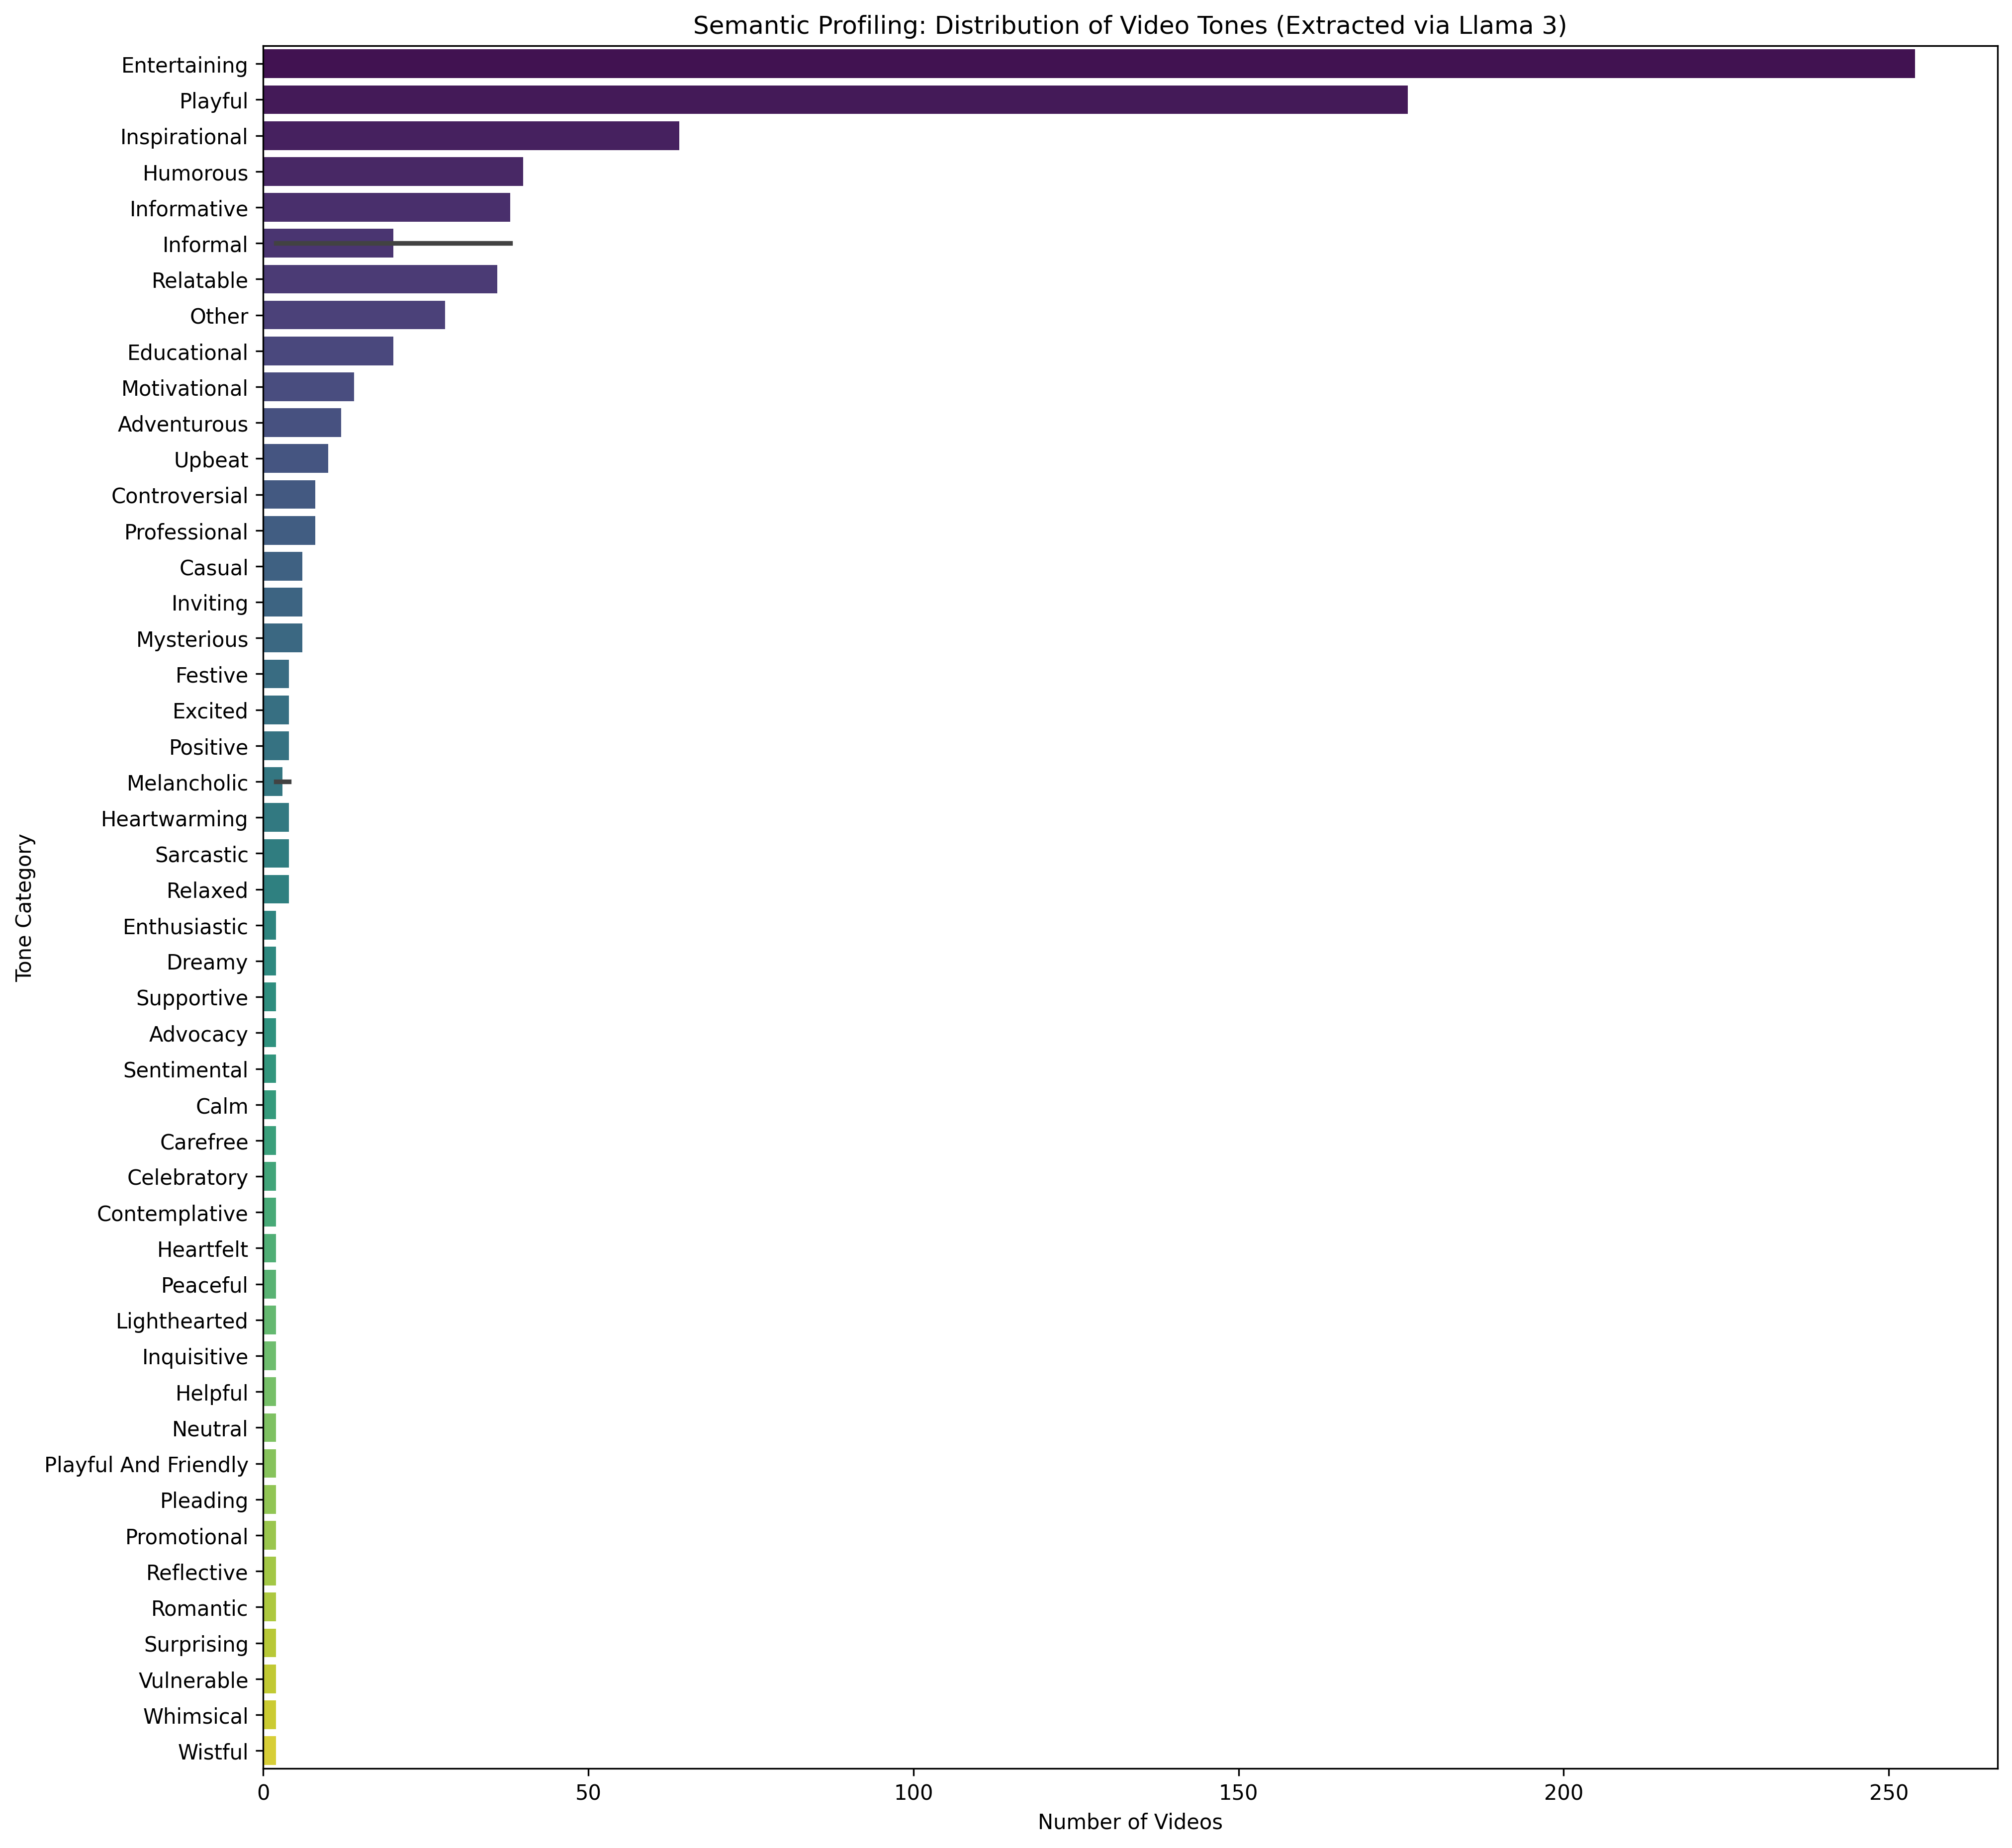
\includegraphics[width=0.75\textwidth]{images/llm_tone_distribution.png}
    \caption{Distribution of video tones extracted via Llama 3 semantic profiling.}
    \label{fig:llm_tone}
\end{figure}

\subsection{Speech-to-Text and Captioning Pipeline}
To maximize accessibility and engagement, we built a transcription and captioning module powered by Whisper. Audio is extracted as 16 kHz mono WAV, and \texttt{faster-whisper} generates word‑level timestamps. Captions are exported as SRT and then converted to ASS for advanced styling, including dynamic font scaling based on word length to ensure readability on 9:16 vertical videos. The final captions are burned into the video using FFmpeg, producing social‑ready, accessibility‑friendly content.

\subsection{Dimensionality Reduction (PCA)}
OpenAI CLIP produces 512‑dimensional embeddings for every video segment. While this rich representation captures fine‑grained visual semantics, it is too high‑dimensional for our dataset and would cause the model to overfit noise instead of learning general patterns.\\  We therefore apply Principal Component Analysis (PCA), which projects the embeddings into a lower‑dimensional subspace that preserves maximal variance. This reduces complexity, improves generalization, and significantly lowers computational cost without discarding the most informative visual signals.

\begin{figure}[H]
    \centering
    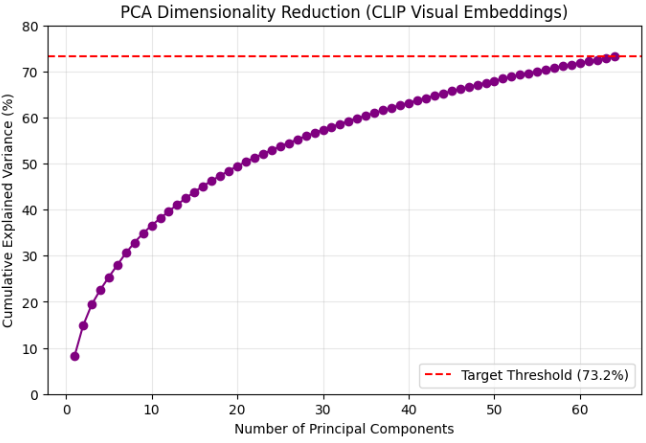
\includegraphics[width=0.6\textwidth]{images/pca_elbow_curve.png}
    \caption{PCA Cumulative Explained Variance for CLIP visual embeddings.}
    \label{fig:pca_elbow}
\end{figure}

Figure \ref{fig:pca_elbow} shows the cumulative explained variance of PCA applied to 512‑D CLIP embeddings. The curve rises quickly in the first components and gradually flattens, indicating diminishing returns. Selecting 64 components preserves approximately 73.4\% of the original variance, which is a strong trade‑off between compression and information retention. This reduces the risk of overfitting on a relatively small dataset while still keeping the most informative visual signals.\\

After dimensionality reduction, we also computed the cosine similarity between hook and full‑video embeddings to quantify visual consistency across the clip.

\begin{figure}[H]
    \centering
    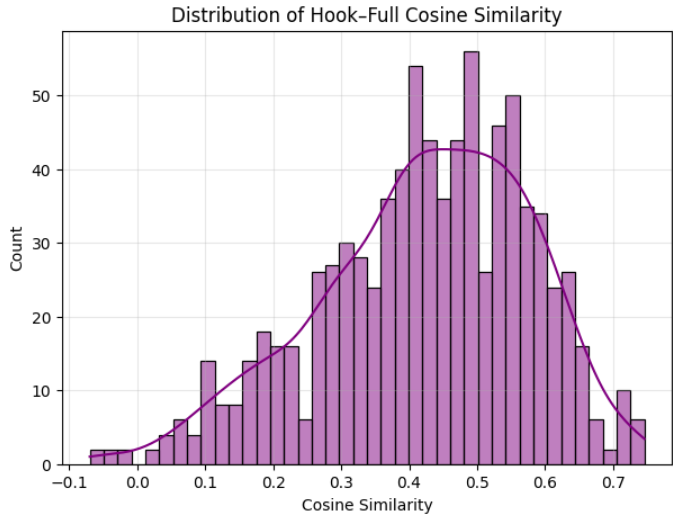
\includegraphics[width=0.6\textwidth]{images/hook_full_cosine_distribution.png}
    \caption{Distribution of cosine similarity between hook and full-video CLIP embeddings.}
    \label{fig:hook_full_cosine}
\end{figure}

Figure \ref{fig:hook_full_cosine} presents the distribution of cosine similarity between hook and full‑video embeddings. Most videos cluster around 0.4–0.6, meaning their opening visual style is moderately consistent with the rest of the content. Low similarity suggests that the hook does not match the main video, which may harm viewer retention, while very high similarity indicates strong visual coherence.
% ══════════════════════════════════════════════════════════════
\subsection{Preprocessing and Feature Engineering Design}

Data preprocessing is heavily customized for multimedia files:
\begin{itemize}
    \item \textbf{Multimodal Slicing:} Raw \texttt{.mp4} videos are programmatically separated into an audio track (\texttt{16kHz} mono \texttt{.wav} for Whisper/Librosa) and visual frames (\texttt{ffmpeg \%06d.png} format). For the predictive agent, the video is further sliced into the "Hook" (first 3 seconds) and the "Full Video" to independently assess user retention strategies.
    \item \textbf{Feature Aggregation:} The predictive agent aggregates the PCA vectors, Llama 3 categorical tags (One-Hot Encoded), and Librosa acoustic metrics into a flat, 473-dimensional dense matrix. 
    \item \textbf{Computer Vision Pre-Filtering:} Before passing frames to the heavy GANs, the system calculates Laplacian variance (blur) and Gaussian deltas (noise). Based on these thresholds, frames are routed through classical OpenCV filters (e.g., Bilateral Filtering with \texttt{d=9, sigma=75}) to remove digital artifacts, ensuring the GANs upscale clean data.
\end{itemize}
\subsection{AI Video Enhancement Pipeline (Optional Module)}
Although the core contribution is prediction, we implemented a separate AI enhancement pipeline to improve video quality before publishing. Each uploaded video is decomposed into frames and audio using FFmpeg. A quality analyzer measures blur (Laplacian variance), noise, and low‑light percentage across sampled frames. Based on these scores, the system auto‑selects a classical filter (bilateral or unsharp mask) to remove artifacts before AI restoration.

The enhancement stage applies a two‑model cascade: (1) Real‑ESRGAN for super‑resolution and texture reconstruction, and (2) GFPGAN for facial restoration when faces are detected. Enhanced frames are reassembled into an H.264 video using CRF‑18 and \texttt{-movflags +faststart} for immediate web playback. The pipeline also computes objective metrics (PSNR, SSIM, LPIPS) to quantify improvement and generates before/after previews for creators.
\subsection{Hyperparameter Configuration}

The models were fine-tuned to balance computational speed and output quality:

\begin{itemize}
    \item \textbf{Predictive Agent (XGBoost \& PCA):} The visual embeddings from CLIP (512D) and NLP embeddings from MiniLM (384D) were compressed using PCA with \texttt{n\_components} set to 64 and 48, respectively. The XGBoost regressor was configured with \texttt{learning\_rate = 0.05}, \texttt{max\_depth = 6}, and \texttt{n\_estimators = 200} to prevent overfitting while maintaining high predictive accuracy.
    \item \textbf{Auto-Captioning (Whisper):} The engine utilizes the \texttt{small} model size, balancing transcription accuracy with processing speed. The \texttt{beam\_size} is set to 5 for optimal decoding, and \texttt{word\_timestamps=True} is strictly enforced to enable dynamic, word-by-word subtitle flashing.
    \item \textbf{Video Enhancement:} Real-ESRGAN is configured with \texttt{scale=4} for ultra-HD upscaling, utilizing a \texttt{tile=512} and \texttt{tile\_pad=10} strategy to prevent GPU Out-Of-Memory (OOM) errors on high-resolution frames. GFPGAN runs on \texttt{version=1.4}. FFmpeg encoding uses a Constant Rate Factor (\texttt{CRF}) of 18 and \texttt{-movflags +faststart} to ensure the final output is pristine and instantly streamable on the web.
\end{itemize}
\section{Model Training and Results}
% ══════════════════════════════════════════════════════════════

The dataset was divided using an 80/20 Train/Test split, ensuring strict deduplication based on \texttt{video\_id} to prevent data leakage. We evaluated multiple models using RMSE, MAE, and $R^2$ scores.

\subsection{Model Choice and Selection Rationale}
To ensure robustness, we compared three strong tree-based regressors widely used for structured, high-dimensional data:
\begin{itemize}
    \item \textbf{XGBoost (XGB):} Known for excellent generalization and strong performance on mixed numerical + categorical features.
    \item \textbf{LightGBM (LGBM):} Optimized for speed and large feature spaces, often competitive with XGBoost.
    \item \textbf{Random Forest (RF):} A reliable baseline ensemble with low variance but weaker performance on complex interactions.
\end{itemize}
To formally evaluate model performance, we computed standard regression metrics defined as follows:

\noindent
\begin{minipage}{0.48\textwidth}
\begin{equation}
\text{MAE} = \frac{1}{n}\sum_{i=1}^{n} \left| y_i - \hat{y}_i \right|
\end{equation}
\end{minipage}
\hfill
\begin{minipage}{0.48\textwidth}
\begin{equation}
\text{RMSE} = \sqrt{ \frac{1}{n}\sum_{i=1}^{n} \left( y_i - \hat{y}_i \right)^2 }
\end{equation}
\end{minipage}

\begin{equation}
R^2 = 1 - \frac{\sum_{i=1}^{n} (y_i - \hat{y}_i)^2}{\sum_{i=1}^{n} (y_i - \bar{y})^2}
\end{equation}

MAE captures average absolute error, RMSE penalizes large deviations, and $R^2$ measures the proportion of variance explained by the model.

\begin{table}[H]
    \centering
    \begin{tabular}{lccc}
        \toprule
        \textbf{Model} & \textbf{RMSE} & \textbf{MAE} & \textbf{$R^2$ Score} \\
        \midrule
        XGBoost (Selected) & \textbf{0.83} & \textbf{0.36} & \textbf{0.85} \\
        LightGBM & 0.90 & 0.42 & 0.82 \\
        Random Forest & 1.12 & 0.78 & 0.73 \\
        \bottomrule
    \end{tabular}
    \caption{Performance comparison of regression models predicting \texttt{log\_views}.}
    \label{tab:model_comparison}
\end{table}

\begin{figure}[H]
    \centering
    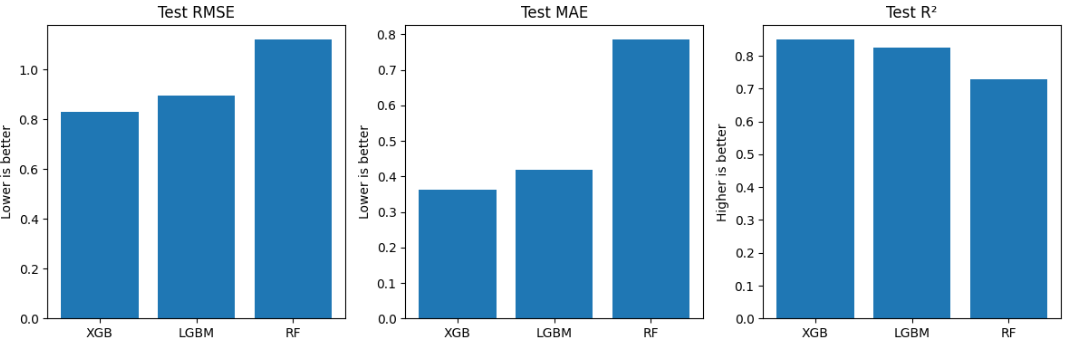
\includegraphics[width=0.9\textwidth]{images/model_comparaison_bars.png}
    \caption{Test set comparison of RMSE, MAE, and $R^2$ across XGBoost, LightGBM, and Random Forest.}
    \label{fig:model_comparison_bars}
\end{figure}

Table \ref{tab:model_comparison}  and Figure \ref{fig:model_comparison_bars}  provide a comparative evaluation across three ensemble models. Although all three perform reasonably well, XGBoost consistently achieves the lowest RMSE and MAE while also delivering the highest $R^2$ score.
\\ LightGBM follows closely but remains inferior in both error metrics, while Random Forest exhibits significantly higher error and lower explanatory power. \\
XGBoost achieved the lowest error and highest $R^2$, making it the most reliable model for deployment. The performance gap is also visible in Figure \ref{fig:model_comparison_bars}, where XGBoost consistently dominates across all three metrics.
\subsection{Results}

\begin{figure}[H]
    \centering
    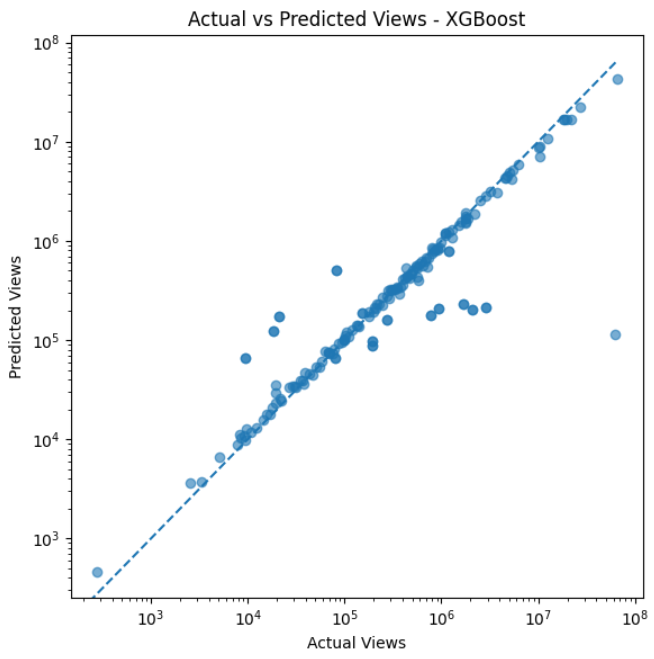
\includegraphics[width=0.4\textwidth]{images/actual_vs_predicted.png}
    \caption{XGBoost Regression Fit: Actual vs. Predicted \texttt{log\_views}.}
    \label{fig:actual_vs_predicted}
\end{figure}

The few deviations from the diagonal correspond to rare viral outliers, which are influenced by external platform dynamics not directly encoded in the video content. Overall, the tight clustering confirms the model’s strong predictive reliability.

% ══════════════════════════════════════════════════════════════
\section{Diagnostics and Explainability}
% ══════════════════════════════════════════════════════════════

\subsection{Learning and Loss Curves}
To prove the model's stability and validate our hyperparameter choices, we generated learning curves and loss curves.

\begin{figure}[H]
    \centering
    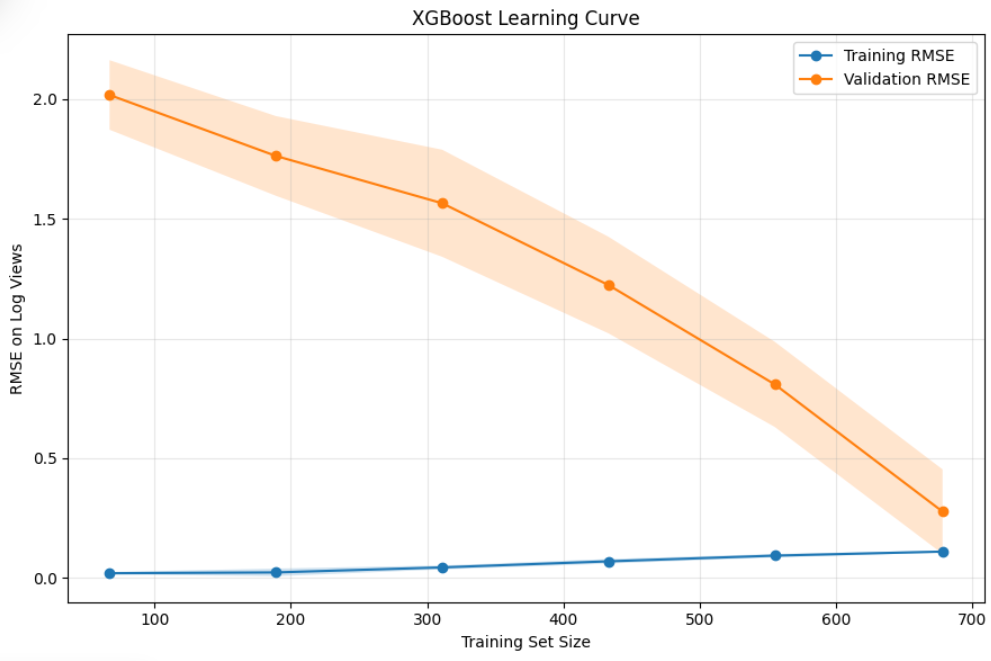
\includegraphics[width=0.6
    \textwidth]{images/learning_curve.png}
    \caption{XGBoost Learning Curve over increasing dataset sizes.}
    \label{fig:learning_curve}
\end{figure}
Figure \ref{fig:learning_curve}  shows a clear generalization trend. The validation RMSE drops consistently as the training size increases, which proves that model performance is data-limited rather than architecture-limited. The shaded band (variance) narrows with larger datasets, indicating reduced sensitivity to sample selection. This confirms that the dataset size is sufficient to stabilize XGBoost and that adding more data directly improves predictive reliability.
\begin{figure}[H]
    \centering
    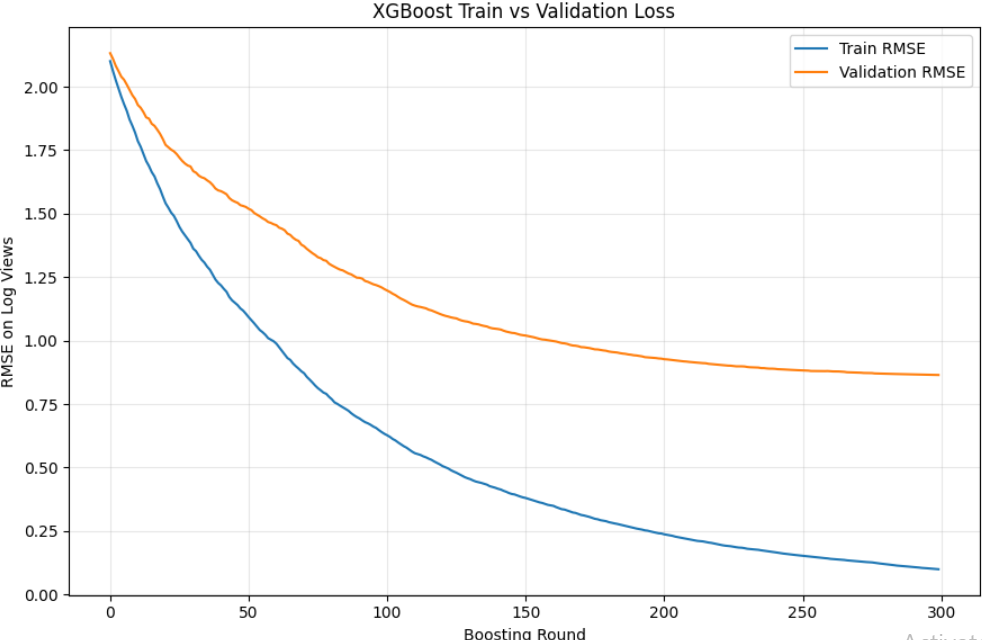
\includegraphics[width=0.6\textwidth]{images/training_loss.png}
    \caption{XGBoost Loss Curve over 300 boosting rounds.}
    \label{fig:training_loss}
\end{figure}

Figure \ref{fig:training_loss} mathematically justifies our data collection efforts; the validation error plunges linearly as more data is introduced. Furthermore, Figure \ref{fig:training_loss} shows smooth convergence without a "U-shape", proving the model does not suffer from late-stage overfitting and justifying the \texttt{n\_estimators=300} limit.
\subsection{Model Explainability (SHAP)}
To provide actionable feedback to content creators, we applied TreeSHAP (SHapley Additive exPlanations), which computes the marginal contribution of each feature to a single prediction. Unlike global feature importance, SHAP explains \emph{why a specific video} is predicted to perform well or poorly by decomposing the final output into positive and negative feature attributions.

In practice, this allows BViral to generate human‑readable advice such as “reduce silence in the first seconds” or “increase hook energy.” It also validates that the model is relying on meaningful signals (e.g., hook embeddings, acoustic energy, and LLM tone categories) rather than spurious correlations. This explainability layer is critical for creator trust and converts the model from a black‑box predictor into a decision‑support agent.

% ══════════════════════════════════════════════════════════════
\section{Critical Discussion \& Architectural Pivot}
% ══════════════════════════════════════════════════════════════
Initially, the project scope included a "Post-Posting" model to predict Engagement Rate. However, our experiments yielded a poor $R^2$ score (0.36) for this metric. Analysis revealed that engagement is heavily influenced by latent external noise (e.g., creator follower count, algorithmic randomization, and time of day) that cannot be extracted from a raw \texttt{.mp4} file. 

Consequently, we made the strategic Data Science decision to drop the Post-Posting model. By scoping down, we focused all compute resources on perfecting the highly reliable \textbf{Pre-Posting Predictive Agent}, ensuring BViral remains a professional, deterministic SaaS tool rather than relying on noisy, uncontrollable post-publication metrics.

\section{Future Improvements}
A major future direction is scaling the dataset. Larger datasets would increase model generalization but require heavier compute resources for feature extraction (CLIP, Whisper, LLM). Future work will therefore allocate stronger GPU/CPU hardware to prevent extraction crashes and to enable batch processing at scale. With more stable infrastructure, we can safely expand the dataset and retrain the model with richer multimodal coverage, potentially improving $R^2$ beyond the current results.
% ══════════════════════════════════════════════════════════════
\section*{Conclusion}
\phantomsection
\addcontentsline{toc}{section}{Conclusion}
% ══════════════════════════════════════════════════════════════
This chapter exhaustively validated the AI methodologies powering BViral Control Center. Through rigorous EDA and the visualization of our multimodal pipeline (PCA, Audio Spectrograms, LLM classification), we proved the complexity of our feature extraction. The XGBoost model successfully mapped these 473 features to achieve an $R^2$ of 0.85, while SHAP integration provided the essential explainability required for a creator-facing agent.
\chapter*{Conclusion \& Perspectives}
\addcontentsline{toc}{chapter}{Conclusion \& Perspectives}

During this end-of-studies project, we designed and developed \textbf{BViral Control Center}, a comprehensive web-based platform that combines multi-platform social media management with AI-powered video enhancement capabilities.

The solution provides content creators with a centralized dashboard to manage their social media presence across YouTube, TikTok, Instagram, and Facebook. Key achievements include:

\begin{itemize}
    \item A modern, responsive React dashboard with real-time analytics, post scheduling via a visual calendar, and comprehensive account management.
    \item A robust Fastify REST API backend with OAuth 2.0 integration (including PKCE for TikTok), AES-256 token encryption, and Supabase Row Level Security.
    \item An automated post publishing pipeline using Redis/BullMQ queues with reliable scheduled delivery and failure handling.
    \item An AI video enhancement pipeline featuring Real-ESRGAN super-resolution, GFPGAN face restoration, and classical filter processing with quality metrics (PSNR, SSIM, LPIPS).
    \item An integrated browser-based video editor (BVIRAL Video Editor) for timeline editing, media import, and export.
    \item A type-safe, full-stack TypeScript monorepo with shared database schemas, API specifications, and Zod validation.
\end{itemize}

This report detailed our approach in three chapters: the state of the art where we analyzed existing solutions and specified requirements; the conceptual study with UML diagrams defining the system's behavior and structure; and the realization chapter covering architecture, technology choices, and implemented interfaces.

\vspace{0.5cm}
\textbf{Future Perspectives:}

While the current implementation achieves its core objectives, several enhancements would further strengthen the platform:

\begin{itemize}
    \item \textbf{Snapchat integration:} extend the OAuth flow to support Snapchat content publishing, completing the five-platform coverage.
    \item \textbf{AI content generation:} integrate large language models for automatic caption, hashtag, and description generation tailored to each platform's best practices.
    \item \textbf{Collaborative workspaces:} add team management features allowing multiple users to collaborate on content calendars with role-based access control.
    \item \textbf{Advanced analytics:} implement predictive analytics using machine learning to forecast post performance and recommend optimal posting times.
    \item \textbf{Mobile companion app:} develop a React Native mobile application for on-the-go scheduling and analytics monitoring.
    \item \textbf{Webhook notifications:} integrate real-time webhook-based notifications from platforms to instantly update post status and analytics.
    \item \textbf{A/B testing:} enable creators to test different captions, thumbnails, or posting times and compare performance across variants.
\end{itemize}


% ---------- References ----------
\begin{thebibliography}{99}
\phantomsection
\addcontentsline{toc}{chapter}{References}

\bibitem{lecun2015}
Y. LeCun, Y. Bengio, and G. Hinton, ``Deep learning,'' \textit{Nature}, vol. 521, pp. 436--444, 2015.

\end{thebibliography}

% ---------- Appendices ----------
\appendix
\input{appendices/installation-guide}
\input{appendices/additional-diagrams}
\input{appendices/api-documentation}

\end{document}
